%%%%%%%%%%%%%%%%%%%%%%%%%%%%%%%%%%%%%%%%%%%%%%%%%%%%%%%%%%%%%%%%%%%%%%%%%%%
%%%%%%%%%%%%%%%%%%%% SVN IN 30 MINUTES - DOCUMENT FILE %%%%%%%%%%%%%%%%%%%%
%%%%%%%%%%%%%%%%%%%%%%%%%%%%%%%%%%%%%%%%%%%%%%%%%%%%%%%%%%%%%%%%%%%%%%%%%%%


\section{Introduction}
\label{section:Intro}

Every time you start to work on something, whatever it is, is very useful use a \textit{Version Control System}.


As you can see from the figure \ref{fig:svnIntro} a VCS allows you to manage your files keeping track of all changes (eventually between you and all other users), allowing you to move back and forward to marked points called commit.

A versioning software allows you also other operations like: branching, merging, adding external repositories, locking files, \ldots\newline

\begin{figure}[htbp]
    \centering
    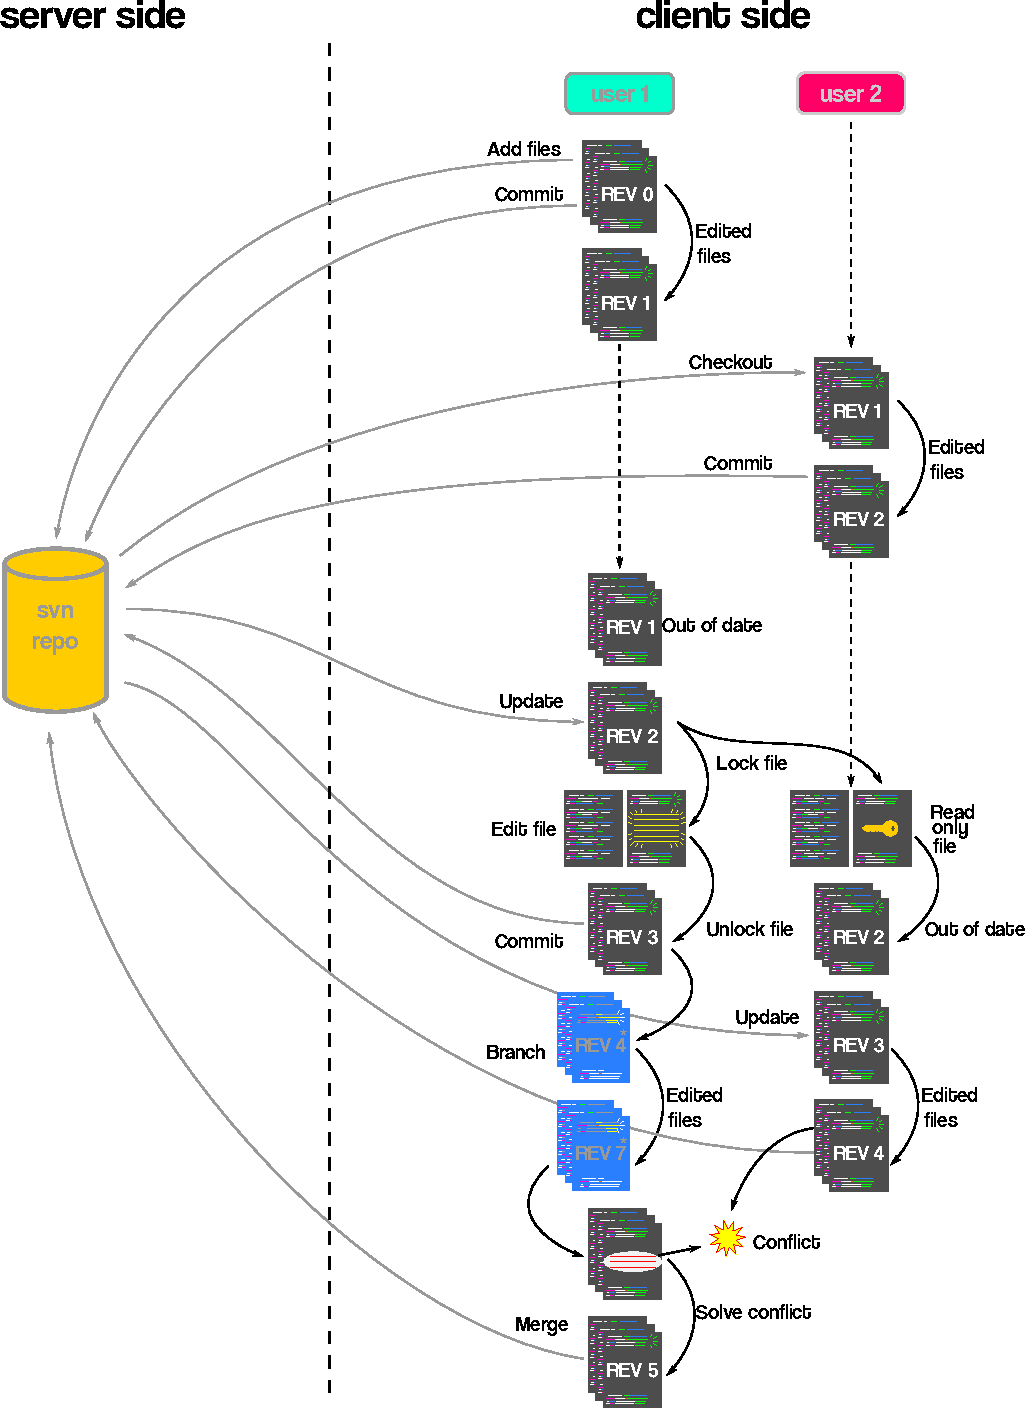
\includegraphics[width=\textwidth, keepaspectratio]{svnIntro.pdf}
    \caption{Typical development work flow using a VCS.}
    \label{fig:svnIntro}
\end{figure}

A complete version control system is divided in two parts\footrednote{See the vertical dashed line in figure \ref{fig:svnIntro}.}: the \textit{server} and the \textit{client} that are normally represented by two separate entities connected through a network connection. \newline

The server is where all operations are executed and where the code within the database\footrednote{In a version control system all operations must be atomic.} is stored, this is why it must be absolutely reliable and guarantee complete data integrity.

The client is where all operations on files are managed and where files are normally used.\newline

In this post I'm going to explain you how to use Apache Subversion, often simply abbreviated as SVN to maintain a project's files under version control system.\newline


I'll guide you from the very beginning to the most used SVN functions.

In the next sections you'll find how:

\begin{itemize}
    \item create a repository;
    \item checkout a repository;
    \item add, commit, update and revert files;
    \item branch, merge code and resolve conflicts;
    \item tag software release;
    \item include externals;
    \item launch command from script;
    \item avoid common mistakes.
\end{itemize}

All examples use the local machine for both the server and client functionality, so there is no need to have another PC on the local network. Of course there is nothing to stop you to execute the server part on a real server machine.\\

Before start with the guide you will need to install the software if not already done.

\subsection{Install the software}
\label{subsection:InstallSoftware}

Download \href{https://tortoisesvn.net/downloads.html}{TortoiseSVN} and install it including the \textit{command line client tools} option (figure \ref{fig:installSVNCmd}) to be able to run the SVN commands from scripts as well.

\begin{figure}[htbp]
    \centering
    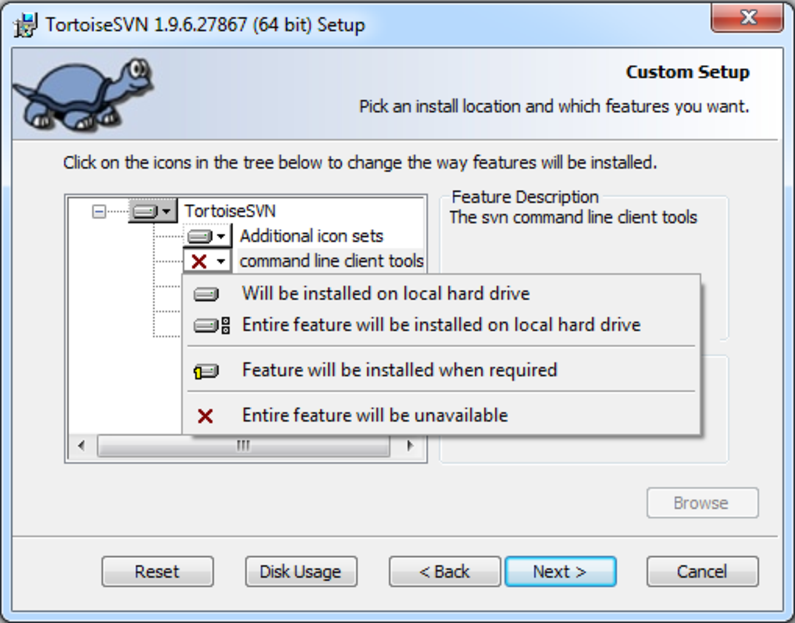
\includegraphics[width=0.6\textwidth, keepaspectratio]{installSVNCommandLine.pdf}
    \caption{Install SVN command line client tool.}
    \label{fig:installSVNCmd}
\end{figure}

If everything has gone well you should have now the TortoiseSVN as a Windows shell extension (figure \ref{fig:shellSVN}).

\begin{figure}[htbp]
    \centering
    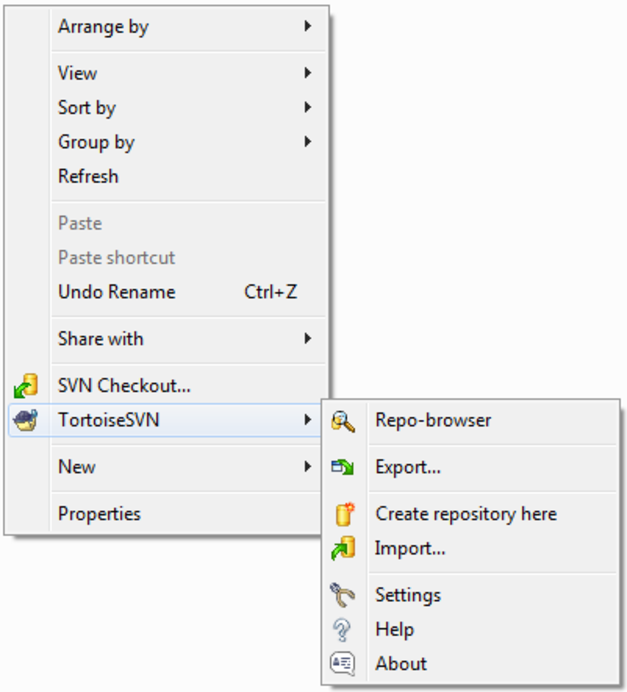
\includegraphics[width=0.5\textwidth, keepaspectratio]{shellSVN.pdf}
    \caption{SVN Windows shell correctly installed.}
    \label{fig:shellSVN}
\end{figure}


\newpage










\section{Setup a project}
\label{section:SetupProject}


To use a version control system on a project you need:

\begin{itemize}

    \item a repository;
    
    \item a working folder.

\end{itemize}

Once you have these two, you can start to develop your project\ldots Let's see how to start.\\


The version control system is like a service that runs on an operating system, it is there, but you can't "see it" until you execute a certain command. To interact with the server you have to send commands from the client using the command line, or a more simple, graphical interface.\\

In this tutorial I'll refer to the popular graphical client TortoiseSVN.






\subsection{Create a repository}
\label{subsection:CreateRepository}



Every project has its own repository, that is the space where the project files will be stored, this is represented by a folder that will contain your committed files\footrednote{Not in an intelligible form.} and auxiliary SVN system files.

Normally it lies on a remote machine\footrednote{As wrote in section \ref{section:Intro} this should be a server. To setup a server check the \href{http://svnbook.red-bean.com/}{official documentation}.}, but to make the example fast to be run, we're going to create it locally.

\begin{itemize}
    \item Choose a directory where execute all the next exercises\footrednote{My root exercise folder is named \textit{Exercises}.} and create another folder (here named \textit{svn repo}) that will be used to contain the repository itself.
    
    \item Select the \textit{svn repo} folder and create the SVN repository: \textit{TortoiseSVN} $\rightarrow$ \textit{Create repository here} (figure \ref{fig:shellCreateRepository}).
    
    \item A pop-up window will appear (figure \ref{fig:repositoryCreated}) to choose which directory structure must be used for the service. Most of the times the default structure will be fine, then press: \textit{Create folder structure}.\\
    Repository is now created with all SVN files needed to manage the versioning service.\\
    A message will confirm the directories creation, and the folder icon will be replaced by a new one (see figure \ref{fig:iconRepository}).
    

\end{itemize}

\begin{figure}[htbp]
    \centering
    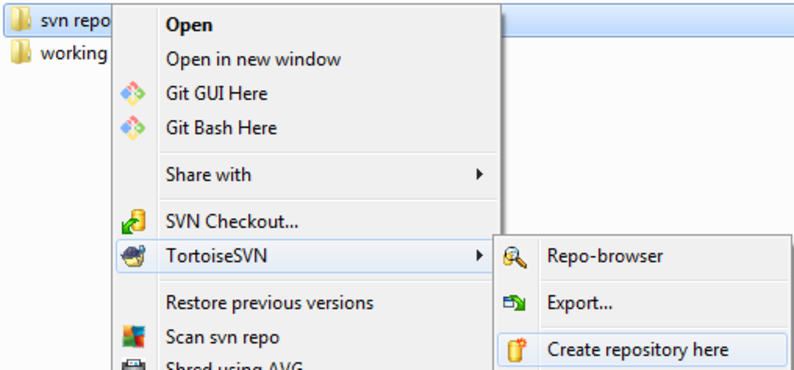
\includegraphics[width=0.6\textwidth, keepaspectratio]{shellCreateRepository.pdf}
    \caption{Create repository with TortoiseSVN.}
    \label{fig:shellCreateRepository}
\end{figure}

\begin{figure}[htbp]
    \centering
    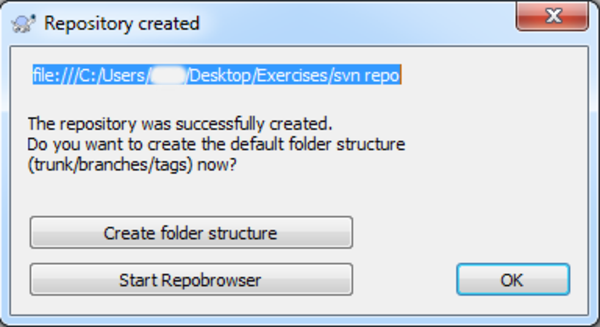
\includegraphics[width=0.5\textwidth, keepaspectratio]{repositoryCreated.pdf}
    \caption{Repository has been created.}
    \label{fig:repositoryCreated}
\end{figure}





\subsubsection{SVN workinkg directory structure}
\label{subsubsection:SVNWorkinkgDirectoryStructure}

If we did not have a version control system, every time we would like test/develop something we should create a temporary folder with the desired branch.
If we had also the necessity to save all the eventually released version we should then create even another folder for every software done. Obviously this procedure, as well as being error prone, will soon led you to a mess in your project.\\

When Subversion initialize the repository it starts by default with three folders: \textit{trunk}, \textit{branches} and \textit{tags} that represent respectively what we call the \textit{working directory}, the \textit{develop directory} and the \textit{release directory}.

These three directories (branches on repository) could be linked to the respective local folders that can have different names, or might point to the same working folder\footrednote{This depends on the development model that you want to use.} and from time to time switch to one of the other (figure \ref{fig:svnDirStructure}). This is by far the most used way.

You can think at the local folder as it would be a "folder shortcut" of the respective safely stored in the repository.

\begin{figure}[htbp]
    \centering
    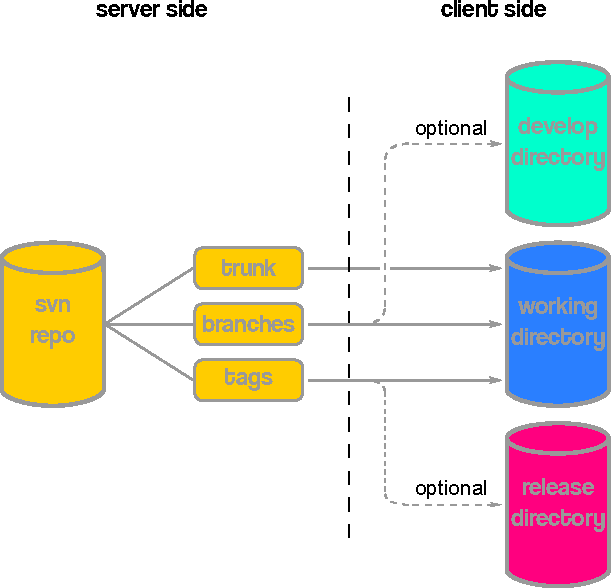
\includegraphics[width=0.6\textwidth, keepaspectratio]{svnDirStructure.pdf}
    \caption{Subversion default folders structure.}
    \label{fig:svnDirStructure}
\end{figure}

Developing code using only the main branch (\textit{trunk}) is not the right way to use the VCS. To make full use of a versioning it is advisable keep on the \textit{trunk} only the software version with complete functions. A branch under the \textit{branches} path should be created when starting to implement a new feature or test some functionality. When a functionality is complete and well integrated it can be then merged back in the main software (\textit{trunk} branch).

Finally the \textit{tags} branch should be used every time that a software is released. This workflow is well depicted in figure \ref{fig:svnWorkflow}.

\begin{figure}[htbp]
    \centering
    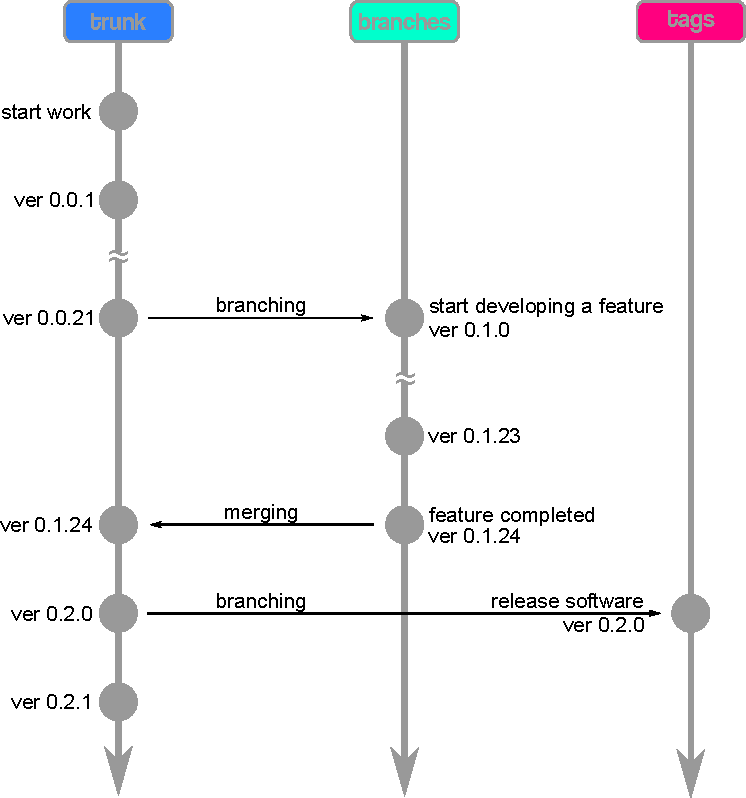
\includegraphics[width=0.6\textwidth, keepaspectratio]{svnWorkflow.pdf}
    \caption{Workflow used with a version control system.}
    \label{fig:svnWorkflow}
\end{figure}

To find out more on this you can read a really nice post (\textit{A successful Git branching model}) on this \href{http://nvie.com/posts/a-successful-git-branching-model/}{blog}.









\subsection{Checkout a repository}
\label{subsection:CheckoutRepo}


All files/folders of a project are normally contained in a root folder (the working directory), to keep it under version control system, it is necessary "connect" this local folder to the repository. As seen this is normally linked to the \textit{trunk} branch in the SVN repository.



\begin{itemize}
    \item Inside the \textit{Exercises} directory create the working folder (here named \textit{working}).

    \item Select that directory and with right click choose: \textit{SVN Checkout...} (figure \ref{fig:shellCheckout}).
\end{itemize}


\begin{figure}[htbp]
    \centering
    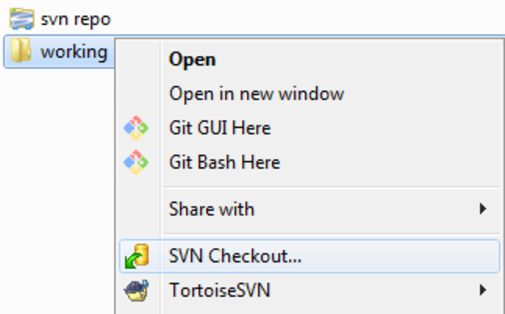
\includegraphics[width=0.45\textwidth, keepaspectratio]{shellCheckout.pdf}
    \caption{Checkout repository to local folder.}
    \label{fig:shellCheckout}
\end{figure}


\begin{itemize}
    \item A pop-up window will appear (figure \ref{fig:svnCheckout}) to let you select both the repository url and the checkout folder. In the \textit{URL of the repository} field insert the path to the repository directory \textit{svn repo} and then select the \textit{trunk}. You can use the repo-browser (using the button beside the textbox) to navigate the repository tree.
    
    \item In the \textit{Checkout directory} field insert the working path (should already be correct).
    
    \item Then confirm the checkout.
\end{itemize}


\begin{figure}[htbp]
    \centering
    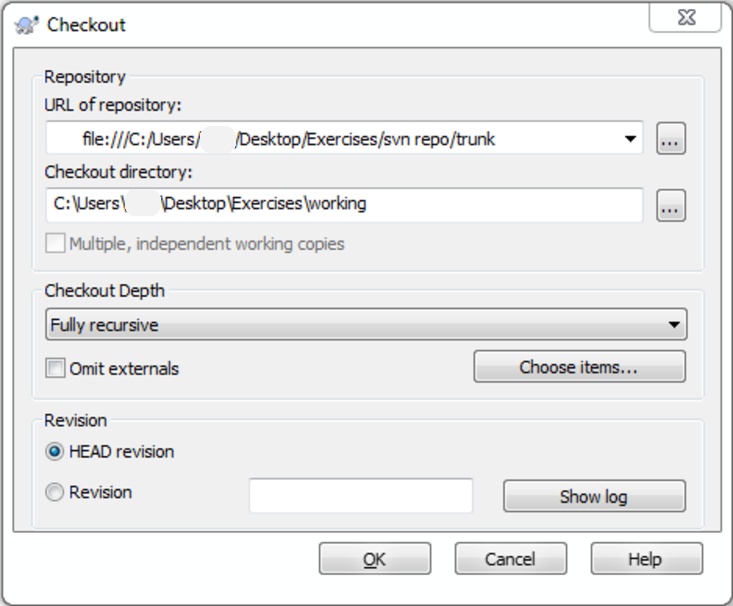
\includegraphics[width=0.55\textwidth, keepaspectratio]{svnCheckout.pdf}
    \caption{Checkout trunk directory.}
    \label{fig:svnCheckout}
\end{figure}


If everything has been done correctly a successful message window will appear (figure \ref{fig:checkoutCompleted}) to confirm you that "the link" between server and client has been established.

\begin{figure}[htbp]
    \centering
    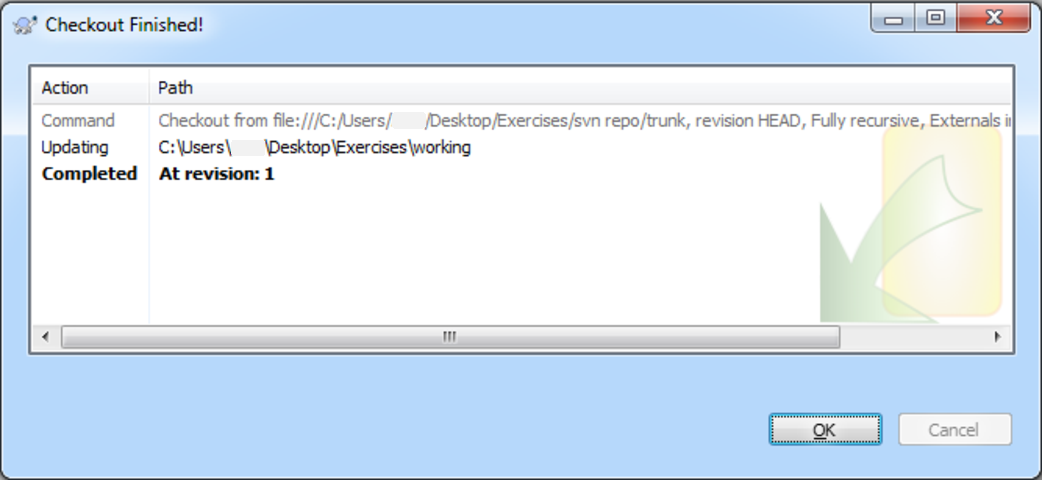
\includegraphics[width=0.75\textwidth, keepaspectratio]{checkoutCompleted.pdf}
    \caption{Checkout successfully completed.}
    \label{fig:checkoutCompleted}
\end{figure}

Now the working directory is under SVN version control and this is showed by the new icon (figure \ref{fig:iconWorkingUpdated}).

\begin{figure}[htpb]
\begin{subfigure}{0.45\textwidth}
  \centering
  
\includegraphics[width=0.26\linewidth, keepaspectratio]{iconSubversion.pdf}
  \caption{SVN repository icon.}
  \label{fig:iconRepository}
\end{subfigure}%
\begin{subfigure}{0.45\textwidth}
  \centering
  
\includegraphics[width=0.25\linewidth, keepaspectratio]{iconUpdated.pdf}
  \caption{Working dir is updated with its repository.}
  \label{fig:iconWorkingUpdated}
\end{subfigure}
\caption{SVN system icons.}
\label{fig:systemIcons_1}
\end{figure}


\newpage











\section{Working on a project}
\label{section:WorkOnProject}

When you start a project, you normally create and/or copy some files to the working folder.

Every time you make changes into files, of course these are saved, but what about if you would have liked to see something that you had and then has been changed?

In the course of time your project grow with new files, how can you check when these were been added to the project?

As you can see in figure \ref{fig:svnCommitWorkflow}, version control systems allow the user to manage all these aspects; in the following section will be presented the necessary commands to interact with the repository.



\begin{figure}[htbp]
    \centering
    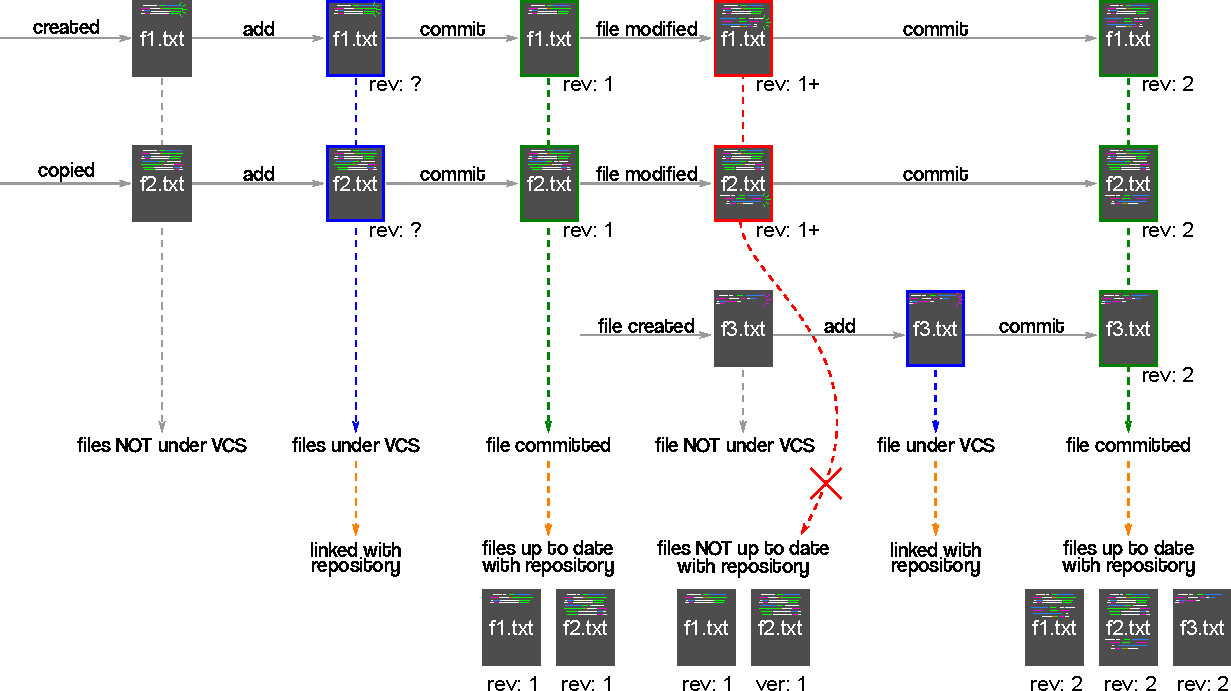
\includegraphics[width=\textwidth, keepaspectratio]{svnCommitWorkflow.pdf}
    \caption{Commit timeline of the project.}
    \label{fig:svnCommitWorkflow}
\end{figure}

\subsection{Adding files}
\label{subsection:AddingFiles}

As you start a project you have to create and/or copy a certain number of files. No matter what is the action made, it is always necessary to inform SVN which files it does need to consider.

\underline{It is not enough just insert files in the working directory}, in fact sometimes the user doesn't want keep track of all files, i.e. temporary files, auto-generated files etc.

This is the reason why versioning software lets the user decide which files are to be included in the compilation.

\begin{itemize}
    \item In this example I'm going to create/copy 2 text\footrednote{Of course they can be any files type.} files: \textit{f1.txt} end \textit{f2.txt} in the working directory. They will appear with a new icon that means that they are not under version control system (figure \ref{fig:iconNotVersioned}).
    
    \item To include them in the version control, select all files and with right click choose:
    \textit{TortoiseSVN} $\rightarrow$ \textit{Add} (figure \ref{fig:svnAdd}). Now these files will be added to SVN and this is showed by the new file icon (figure \ref{fig:iconAdded}).
\end{itemize}


\begin{figure}[htbp]
\begin{subfigure}{0.5\textwidth}
  \centering
  
\includegraphics[width=0.15\linewidth, keepaspectratio]{iconNotVersioned.pdf}
  \caption{Files not under VCS.}
  \label{fig:iconNotVersioned}
\end{subfigure}%
\begin{subfigure}{0.5\textwidth}
  \centering
  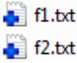
\includegraphics[width=0.15\linewidth, keepaspectratio]{iconAdded.pdf}
  \caption{Files added to a VCS.}
  \label{fig:iconAdded}
\end{subfigure}
\caption{SVN icons for files in a checkout directory.}
\label{fig:systemIcons_2}
\end{figure}


\begin{figure}[htbp]
    \centering
    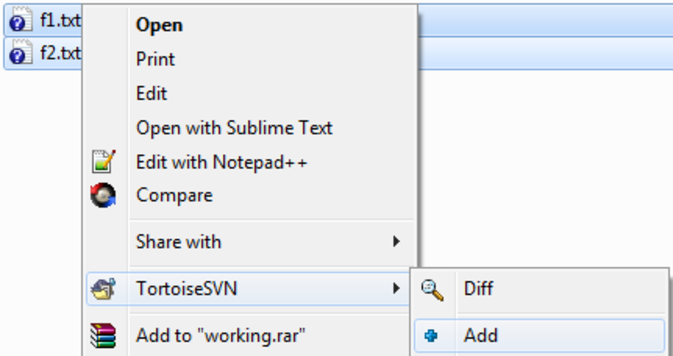
\includegraphics[width=0.6\textwidth, keepaspectratio]{shellAdd.pdf}
    \caption{Add project files into the SVN repository.}
    \label{fig:svnAdd}
\end{figure}

To safely store the added files to the repository we need one more operation: the commit.










\subsection{Commit files}
\label{subsection:CommitFiles}

Commit can be thought as a point where something important happens, so it must be possible to return whenever will be necessary.

This operation allows the user, through the client, to store these files on the repository, associating files with a unique number accompanied by a descriptive user message.

Figure \ref{fig:svnCommitWorkflow} shows a typical project workflow: files are first added, then the changes are committed to the repository.\\



\begin{itemize}
    \item To commit a project, select the added files or the working dir, then right click and choose \textit{SVN Commit\ldots} (figure \ref{fig:shellCommit}).
    
    \item In the window summary (figure \ref{fig:commitMessage}) insert the commit comment related to the modified files. It is important use a self-explanatory comment\footrednote{See the subsection \ref{subsubsectio:HowWriteRevision}.} in order to be able to remember the state of the project at the $x$ commit.
    
    
\end{itemize}

\begin{figure}[ht!]
    \centering
    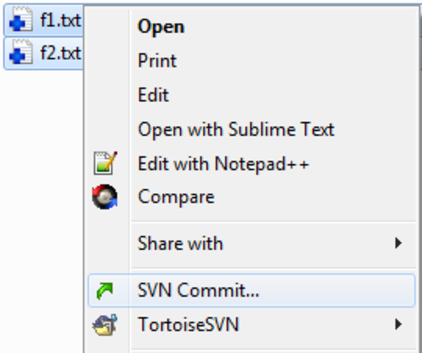
\includegraphics[width=0.35\textwidth, keepaspectratio]{shellCommit.pdf}
    \caption{Commit project files.}
    \label{fig:shellCommit}
\end{figure}



\begin{figure}[ht!]
    \centering
    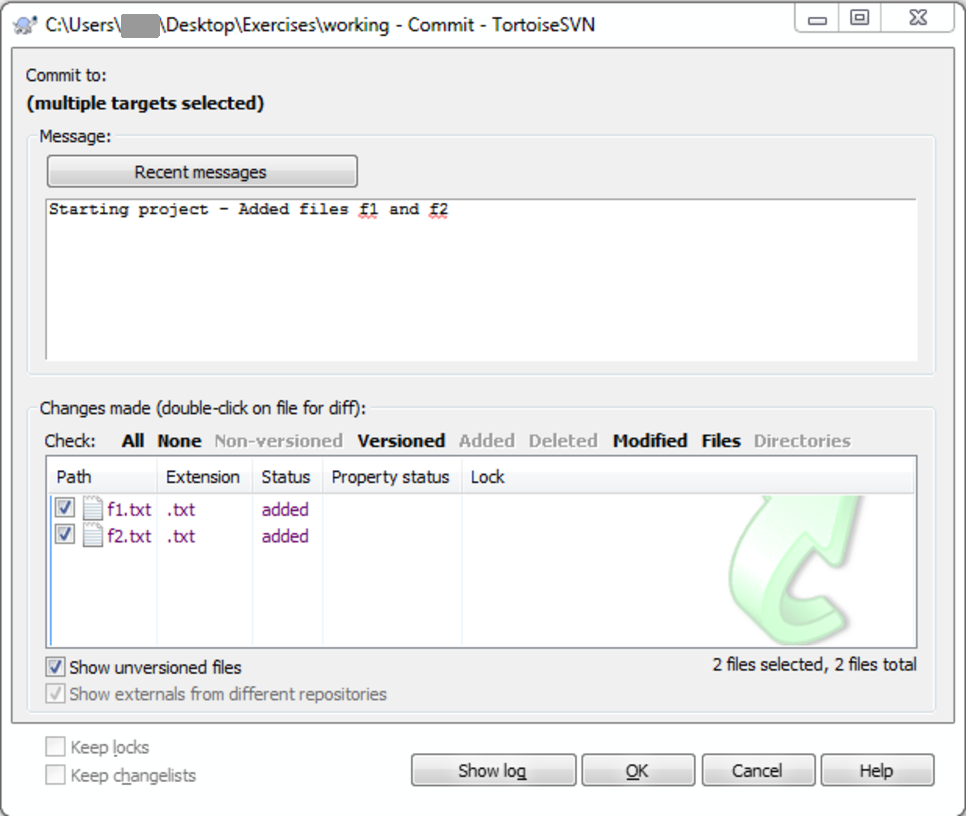
\includegraphics[width=0.65\textwidth, keepaspectratio]{commitMessage.pdf}
    \caption{Commit window with the user message.}
    \label{fig:commitMessage}
\end{figure}


If everything has been done correctly a successful message window will appear (like figure \ref{fig:checkoutCompleted}) to confirm the operation. Now files icon should look like in figure \ref{fig:iconFilesUpdated}.\\

Suppose now that to add some functionality to our first function we need to modify the two previous files and add a new one; the situation will appear as in the figure \ref{fig:iconModified}.

We see that \textit{f1.txt} and \textit{f2.txt} have been modified, while \textit{f3.txt} has been only added to the project directory. If we want that it would be part of the project we need to add it as previously done with \textit{f1.txt} and \textit{f2.txt}.\\

At the end of the operation, the folder contents will be represented as in figure \ref{fig:iconCommit}.

Now as you may have guessed, to store and sync the modified files to the repository it is necessary execute the commit operation (figure \ref{fig:svnCommitWorkflow}).\\

Again, if everything has worked properly SVN will ask to the user to insert an explanatory commit message as seen before (figure \ref{fig:commitMessage}).

\begin{figure}[htbp]
\begin{subfigure}{0.33\textwidth}
  \centering
  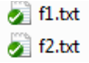
\includegraphics[width=0.3\linewidth, keepaspectratio]{iconFilesUpdated.pdf}
  \caption{} %Files commited and updated with the repository.
  \label{fig:iconFilesUpdated}
\end{subfigure}%
\begin{subfigure}{0.33\textwidth}
  \centering
  
\includegraphics[width=0.25\linewidth, keepaspectratio]{iconModified.pdf}
  \caption{}%Files modified and third file created.
  \label{fig:iconModified}
\end{subfigure}
\begin{subfigure}{0.33\textwidth}
  \centering
  
\includegraphics[width=0.25\linewidth, keepaspectratio]{iconCommit.pdf}
  \caption{}%Third file added to the VCS.
  \label{fig:iconCommit}
\end{subfigure}
\caption{SVN icons during the project evolution.}
\label{fig:systemIcons_3}
\end{figure}

\newpage









\subsection{Update files}
\label{subsection:UpdateFiles}

When you work on a common project all files can be edited by anyone in your group, so before you start to work, you have to update your local copy to reflect the changes in the repository that maybe someone did.

If someone change and commit a certain file, your local copy is not more up-to-date with the project development. If you edited the same file without updating your local copy first, you could end up with a conflict (figure \ref{fig:svnUpdateFlow}).\\


\begin{figure}[htbp]
    \centering
    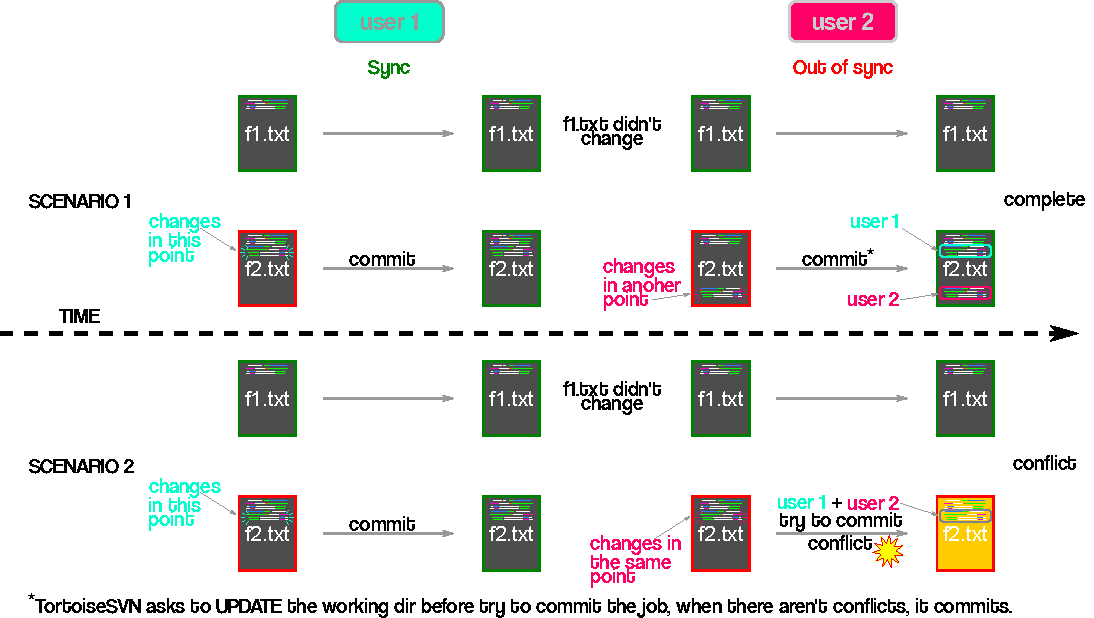
\includegraphics[width=\textwidth, keepaspectratio]{svnUpdateFlow.pdf}
    \caption{When the user doesn't keep the working dir up-to-date he can get in trouble.}
    \label{fig:svnUpdateFlow}
\end{figure}


If users do changes to the same file, versioning systems can understand if the changes done are compatible, and in that case it is going to "merge" both.\\




When the changes aren't compatible (for example both users edit the same function), the versioning systems can't decide which are the right files part to keep, or to merge. In this case you'll end up with a conflict that the user must resolve to be able to commit the project.\\




To update your working directory:

\begin{itemize}

    \item Select the project folder, then choose \textit{SVN Update} (figure \ref{fig:shellUpdate}).
    
    \item If the process complete correctly, a new window will confirm you that both local and repository copies are up to date to a certain revision number.

\end{itemize}




\begin{figure}[htbp]
\begin{subfigure}{0.48\textwidth}
  \centering
  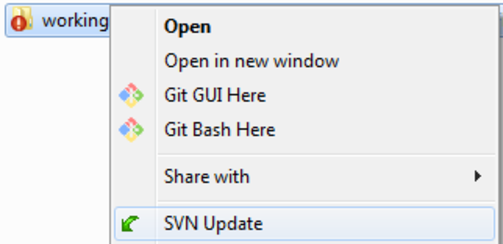
\includegraphics[width=0.75\linewidth, keepaspectratio]{shellUpdate.pdf}
  \caption{}
  \label{fig:shellUpdate}
\end{subfigure}%
\begin{subfigure}{0.48\textwidth}
  \centering
  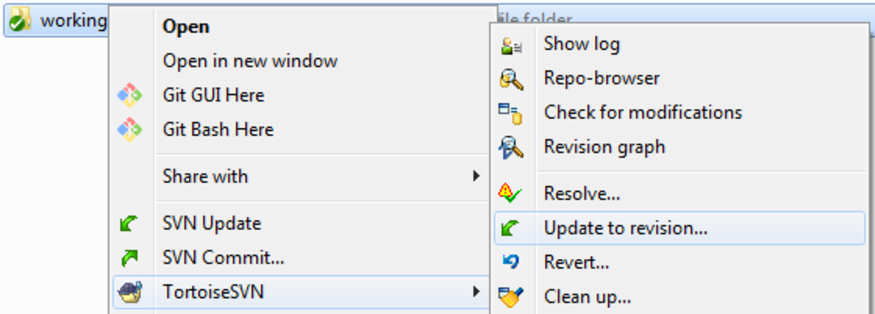
\includegraphics[width=1.1\linewidth, keepaspectratio]{shellUpdateToRevision.pdf}
  \caption{}
  \label{fig:shellUpdateToRevision}
\end{subfigure}
\caption{The update allows the user to sync his local revision with the last on the repository. With the update to revision, the user can move back and forth on the project commits.}
\label{fig:svnUpdate}
\end{figure}


From this point the user can continue to work with the safety of not encountering any conflict.








\subsubsection{Update to release}
\label{subsubsection:UpdateToRelease}


To move back and forward on the project history (commits) the user needs to use the "update to revision" command.\\
\newpage

To update your working directory to the desired version:

\begin{itemize}

    \item Select project folder, then choose \textit{TortoiseSVN} $\rightarrow$ \textit{Update to revision...} (figure \ref{fig:shellUpdateToRevision}).
    
    \item A new pop-up window will appear (figure \ref{fig:updateToRevision}), press the \textit{Show log} button to list all the available commits.
    
    \item Select the desired commit from the list (figure \ref{fig:selectCommitRevision}).
    
    The number of the selected revision will appear in the field below the button (figure \ref{fig:updateToRevision}). Finally execute the update. If the process complete correctly, a new window will confirm you that both local and repository copies are up to date to the selected revision.
    
\end{itemize}






\begin{figure}[htbp]
    \centering
    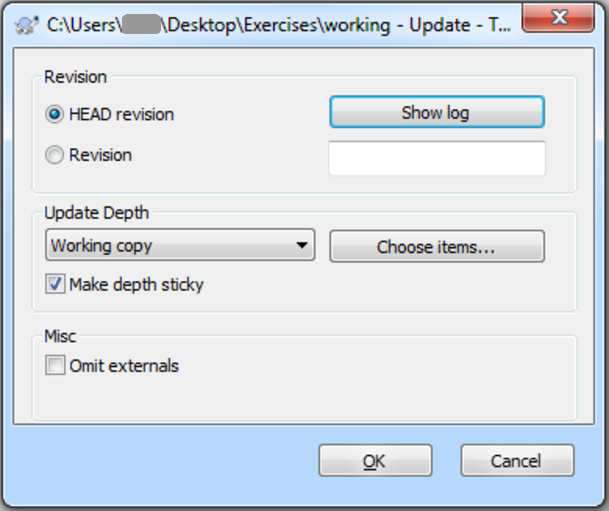
\includegraphics[width=0.45\textwidth, keepaspectratio]{updateToRevision.pdf}
    \caption{The user can select the desired commit using the \textit{Show log} button, or insert the right number in the field below.}
    \label{fig:updateToRevision}
\end{figure}





\begin{figure}[ht!]
    \centering
    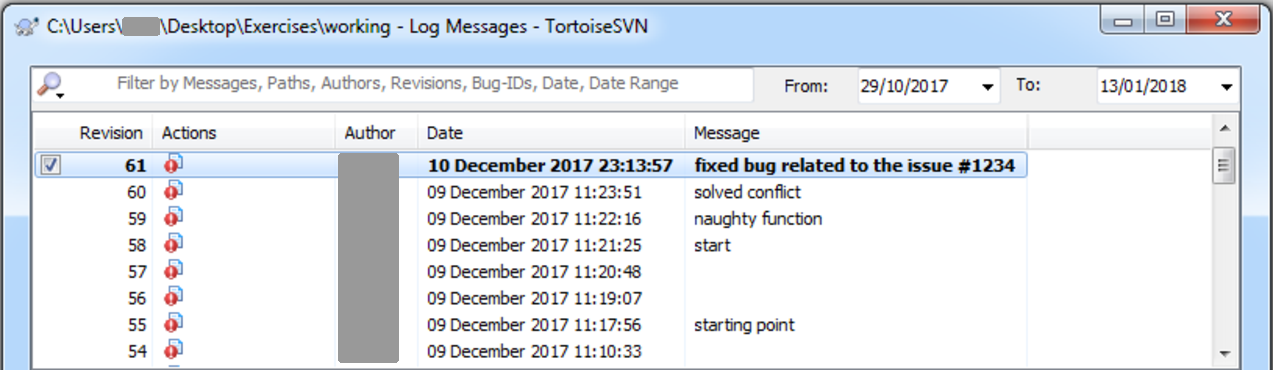
\includegraphics[width=0.9\textwidth, keepaspectratio]{selectCommitRevision.pdf}
    \caption{This window allows the user to select the desired commit.}
    \label{fig:selectCommitRevision}
\end{figure}





To return the project to the last revision just use the \textit{SVN Update} command.

Another useful feature of the \textit{update} command is that we can execute it without the fear that the changes did at the local files would be overwritten. For example you and a your colleague are working at the same project but on different files.
Sometimes you both want to have a peek of each other. Using the update command you will be able to "download" his new version of the file without losing changes that you did in yours.








\subsection{Revert files}
\label{subsection:revertFiles}

The last command of this section, is useful when you want to discard all changes made at the project files and revert to the last revision present in the local folder.\\


For example after committing your project you want to try to fix a bug, but as soon as you start to edit the code, you realise that there is one more important to be fixed first. So, to quickly restart the job, exactly from the last commit, you have to use the revert command.\\


\underline{Pay attention that any "update" command does not discard the changes!} This is a desirable behaviour, since we want to avoid losing any development done in the project when wishing to update remaining project files.\\

If we update 2 files of our example project, but before commit you decide that only one is correct.\\

To discard your changes:


\begin{itemize}

    \item Select the working folder, then with the right click select \textit{TortoiseSVN} $\rightarrow$ \textit{Revert...} (figure \ref{fig:shellRevert}).
    
    \item A pop-up window will appear let you select the modified files to revert (figure \ref{fig:revertFiles}). The selected file will be resetted at the same point where it was at the committing time.

\end{itemize}




\begin{figure}[htbp]
\begin{subfigure}{0.5\textwidth}
  \centering
  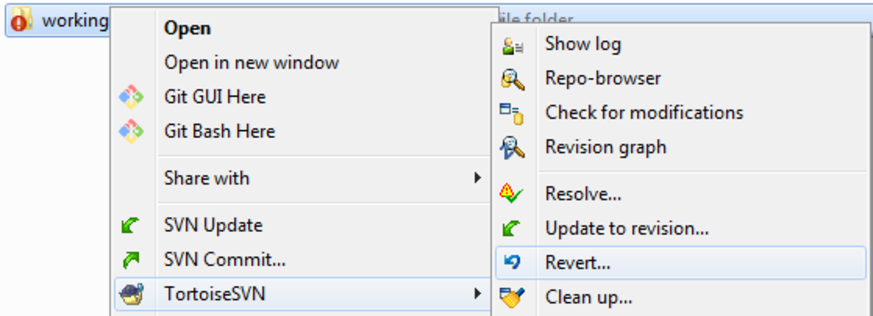
\includegraphics[width=0.95\linewidth, keepaspectratio]{shellRevert.pdf}
  \caption{}
  \label{fig:shellRevert}
\end{subfigure}%
\begin{subfigure}{0.48\textwidth}
  \centering
  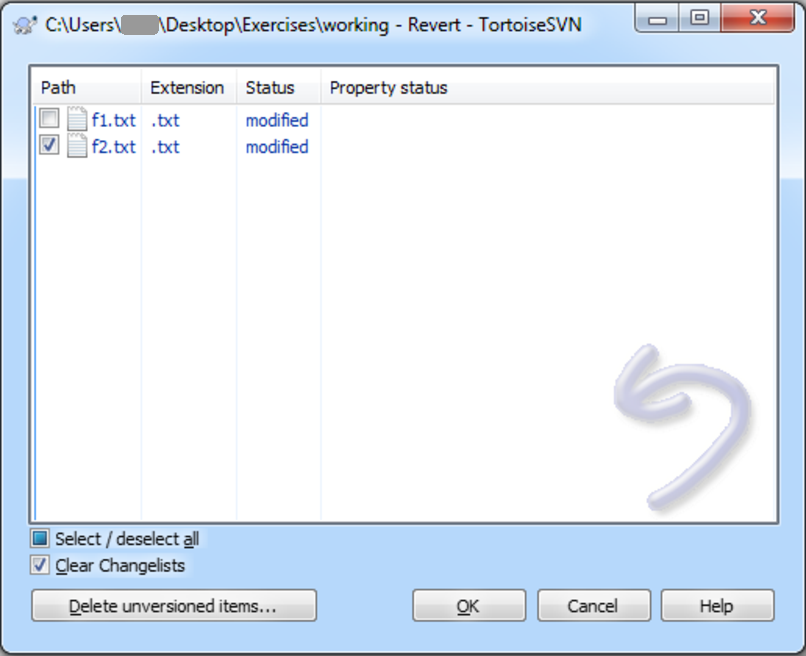
\includegraphics[width=0.85\linewidth, keepaspectratio]{revertFiles.pdf}
  \caption{}
  \label{fig:revertFiles}
\end{subfigure}
\caption{With the revert you can discard all/some changes of the project.}
\label{fig:svnRever}
\end{figure}


\newpage












\section{Branching and merging}
\label{sec:BranchingMerging}


As suggested in the \ref{subsubsection:SVNWorkinkgDirectoryStructure}, the branch can be useful to develop something that we are not ready to insert, or that we are not sure that we want into the main program. Similarly, the merge operation allows the code to be inserted in an existing branch. \newline


\subsection{Branch project}
\label{subsection:branchProject}

Related to our example, suppose that after some work on the project we are ready to add a new functionality (named \textit{niceFunction}).

In this case we might start to develop this function on another branch in order to maintain the \textit{trunk} always as "working" branch.\\


To create a branch for our project:
\begin{itemize}

    \item Select project folder, then choose \textit{TortoiseSVN} $\rightarrow$ \textit{Branch/tag...} option from the menu (figure \ref{fig:shellCreateBranch}), a new pop-up window will appear (figure \ref{fig:addBranch}).
    
    \item To create the branch under the \textit{branches} directory, write into the \textit{To path:} field the desired branch name (figure \ref{fig:addBranch}).\\
    Finally choose the radio button \textit{HEAD revision in the repository} and select the checkbox \textit{Switch working copy to new branch/tag} and complete the operation with a log message.
    
\end{itemize}



\begin{figure}[htbp]
\begin{subfigure}{0.48\textwidth}
  \centering
    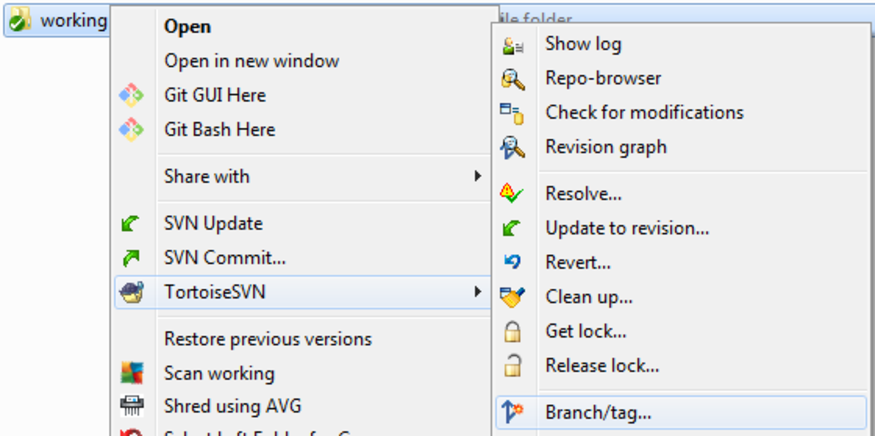
\includegraphics[width=\textwidth, keepaspectratio]{shellCreateBranch.pdf}
    \caption{Create project branch.}
    \label{fig:shellCreateBranch}
\end{subfigure}%
\begin{subfigure}{0.48\textwidth}
  \centering
    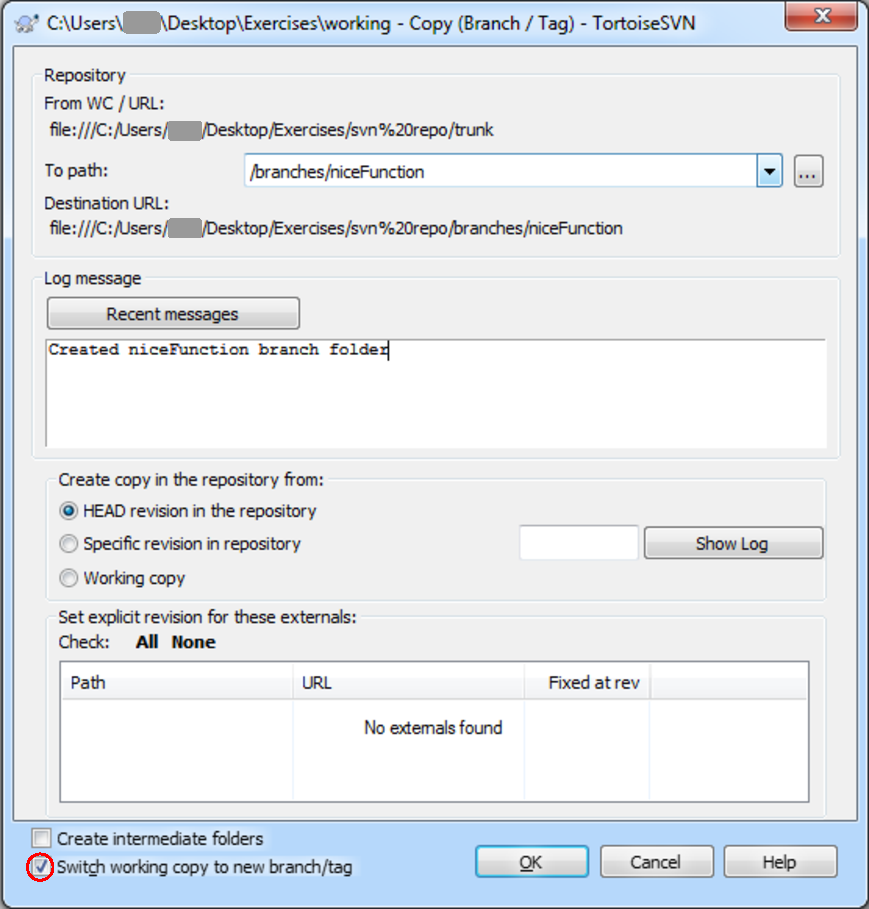
\includegraphics[width=0.9\textwidth, keepaspectratio]{addBranch.pdf}
    \caption{Add branch folder.}
    \label{fig:addBranch}
\end{subfigure}%
\caption{}
\label{fig:switchMakeBranch}
\end{figure}


Now the local folder will be "connected" to this new branch: \textit{niceFunction}, and it is possible start to create the desired function on the branch (figure \ref{fig:svnDirStructure}).














\subsection{Merge a branch}
\label{subsection:shellMergeBranch}

When we want to merge into the main program (the \textit{trunk}) a functionality that comes from another branch or repository, we need to execute the \textit{merge} command.\\


Referring to our example, let's say that we successfully completed the function created in the branch \textit{niceFunction} and then we want to merge it into the main trunk of our project. \\

Be aware that, to successfully execute the merge command it is necessary be on the folder that \underline{will receive} the update. So if we are still in the branch \textit{niceFunction} it is necessary to switch from the local copy to the \textit{trunk}.\\

To merge the example:

\begin{itemize}

    \item  Select the \textit{working} folder and choose \textit{TortoiseSVN} $\rightarrow$ \textit{Switch...} (figure \ref{fig:shellSwitchBranch}).
    
    A new pop-up window will allow you to select where the local folder should be switched to; in this case select the \textit{trunk} (figure \ref{fig:switchToBranch}). 

	
    \item Select the project folder, then choose \textit{TortoiseSVN} $\rightarrow$ \textit{Merge...} option (figure \ref{fig:shellMergeBranch}).
    
	
    \item In the appeared window select the option \textit{Merge two different tree} (figure \ref{fig:mergeWindow1}) and continue.
	
	
	\item A new window will appear (figure \ref{fig:mergeWindow2}) querying to insert the path for the \textit{From:} and for the \textit{To:} fields. This will "sounds" a bit odd, but the first\footrednote{Yes this is not a typo, to find out more press the TortoiseSVN "Help" button.} field needs to be filled with the url of the \textit{trunk}.
	
	Fill the second field with the url of the branch that we want to transfer into the trunk (in this example the \textit{niceFunction}).
	
    
    \item We are finally ready to merge both branches. Before executing the command it is preferable to test it using the dedicated button (figure \ref{fig:mergeWindow3}). At this point two scenarios are possible:
    
    \begin{itemize}
    
    \item there aren't conflicts and the merge complete straightforward;
    
    \item there are conflicts and the user must resolve it to complete the merge.
    
    \end{itemize}

\end{itemize}




\begin{figure}[htbp]
\begin{subfigure}{0.5\textwidth}
  \centering
    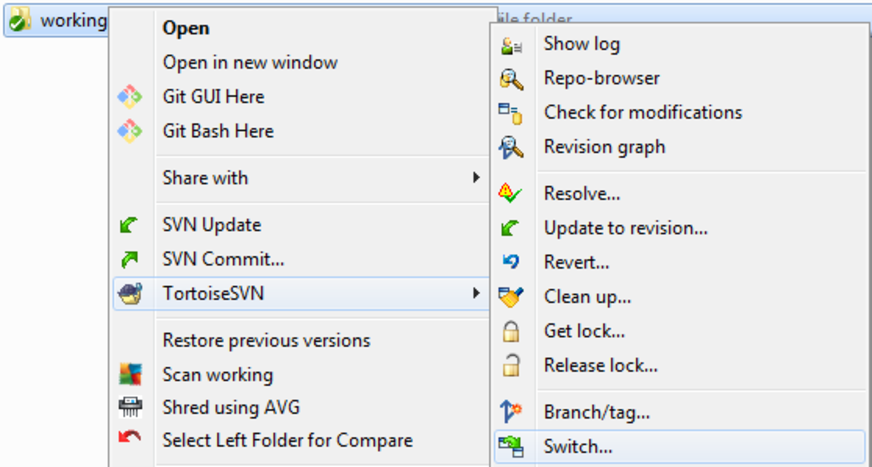
\includegraphics[width=0.8\textwidth, keepaspectratio]{shellSwitchBranch.pdf}
    \caption{Switch to branch menu.}
    \label{fig:shellSwitchBranch}
\end{subfigure}%
%\hspace{2mm}
\begin{subfigure}{0.5\textwidth}
  \centering
    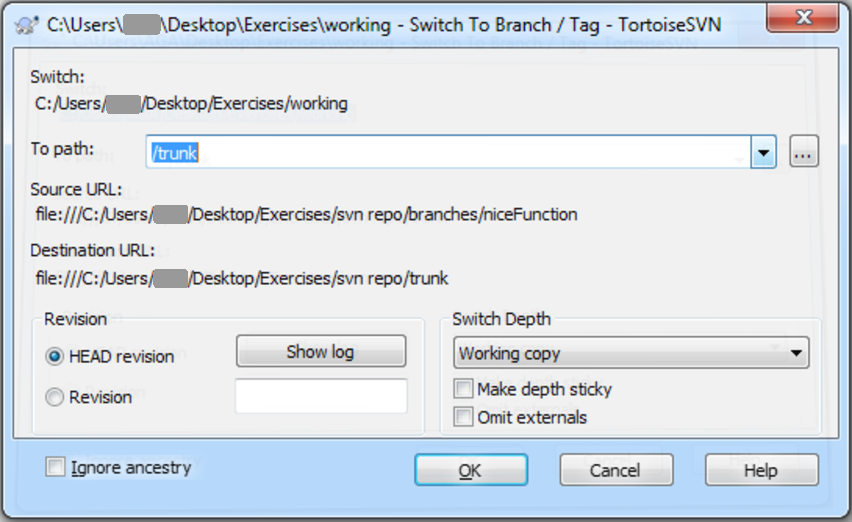
\includegraphics[width=0.7\textwidth, keepaspectratio]{switchToBranch.pdf}
    \caption{Select the trunk branch.}
    \label{fig:switchToBranch}
\end{subfigure}%
\caption{}
\label{fig:switchShells}
\end{figure}




\begin{figure}[htbp]
\begin{subfigure}{0.5\textwidth}
  \centering
    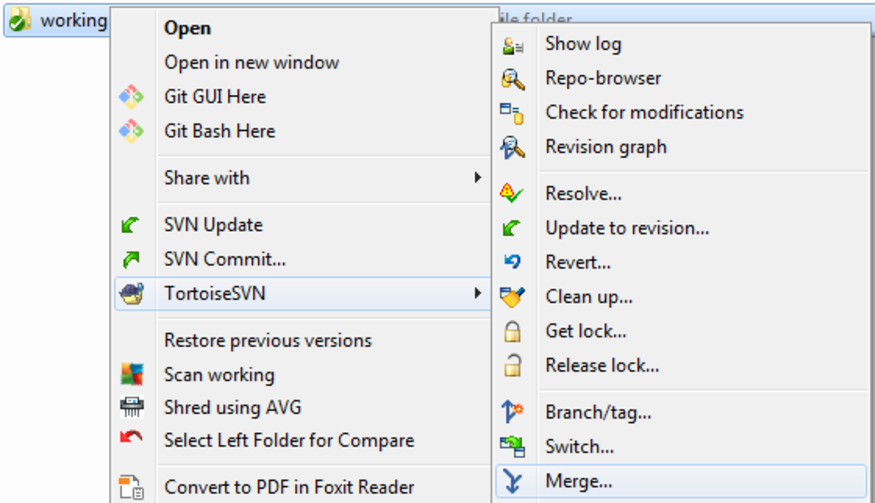
\includegraphics[width=0.8\textwidth, keepaspectratio]{shellMergeBranch.pdf}
    \caption{Merge branch menu.}
    \label{fig:shellMergeBranch}
\end{subfigure}%
%\hspace{2mm}
\begin{subfigure}{0.49\textwidth}
  \centering
    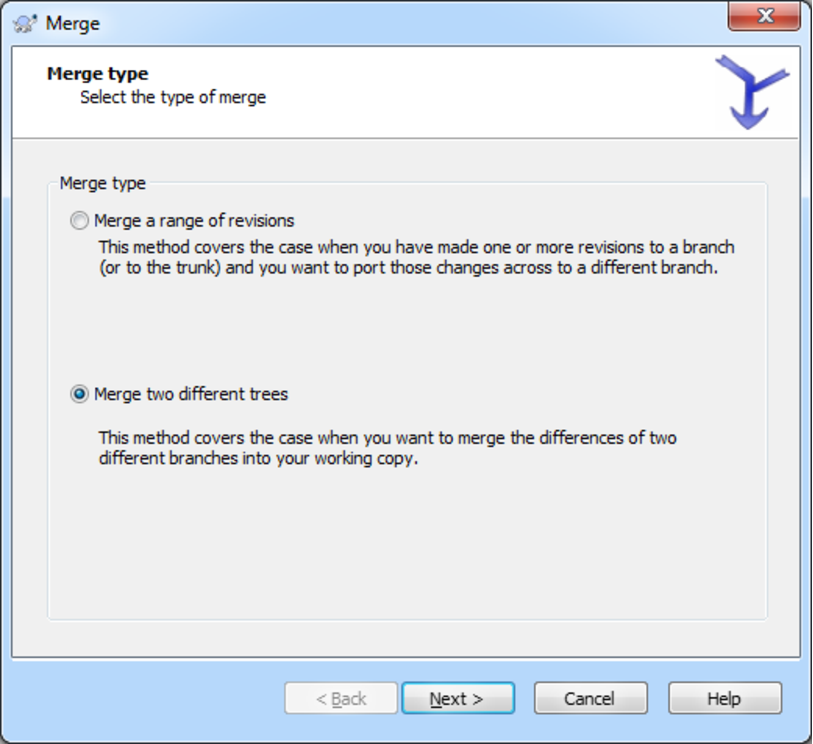
\includegraphics[width=0.6\textwidth, keepaspectratio]{mergeWindow1.pdf}
    \caption{Select the desired merge type.}
    \label{fig:mergeWindow1}
\end{subfigure}%
\caption{}
\label{fig:mergeShells}
\end{figure}




\begin{figure}[htbp]
\begin{subfigure}{0.48\textwidth}
  \centering
  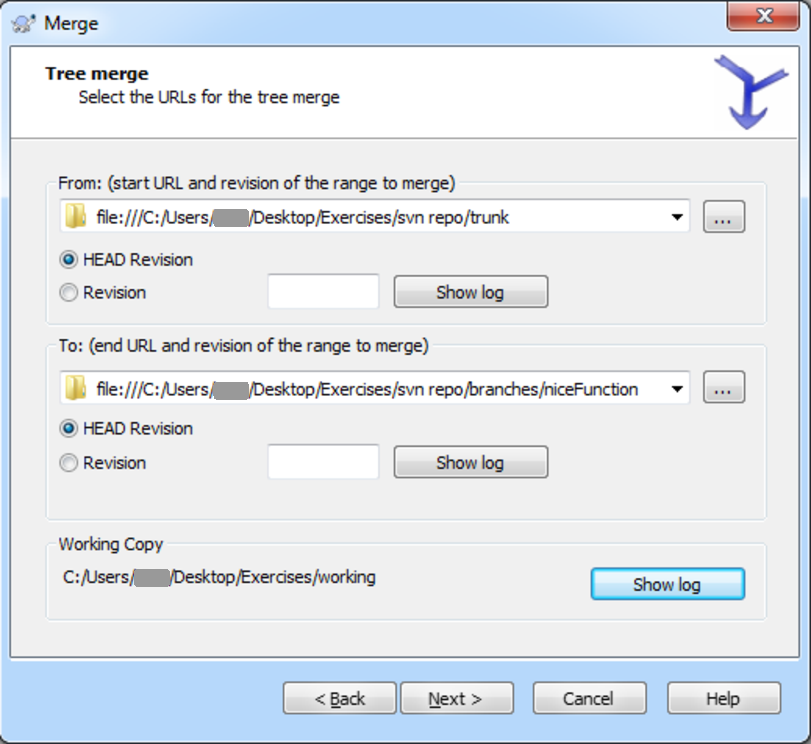
\includegraphics[width=1.025\textwidth, keepaspectratio]{mergeWindow2.pdf}
  \caption{Select the branch to be merged into the \textit{trunk}.}
  \label{fig:mergeWindow2}
\end{subfigure}%
\hspace{2mm}
\begin{subfigure}{0.45\textwidth}
  \centering
  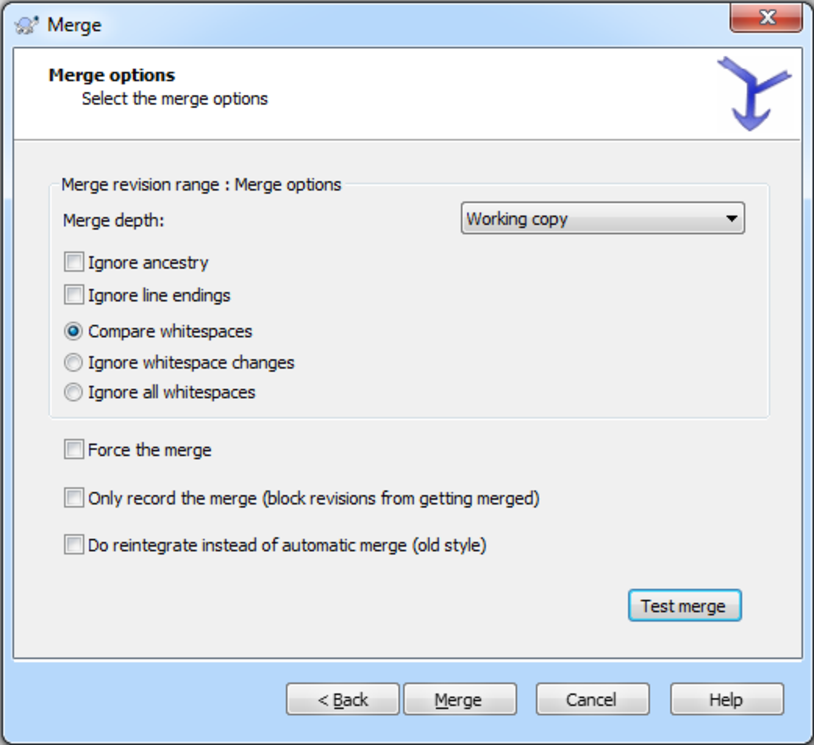
\includegraphics[width=1.1\textwidth, keepaspectratio]{mergeWindow3.pdf}
  \caption{Execute the merge into the \textit{trunk} branch.}
  \label{fig:mergeWindow3}
\end{subfigure}%
\caption{}
\label{fig:mergeWindows}
\end{figure}


In the first case, we can simply execute the command finding the new function \textit{niceFunction} inserted in the main program, while in the second case we need to resolve the conflict to complete the operation.\\


\subsection{Resolve conflicts}
\label{subsection:ResolveConflicts}


A conflict occurs whenever two or more users edit the same document "at the same time", and not seeing one of the changes that the other is making it may overlap. Since the software is not smart enough to decide which of the changes is "correct", it requires the user to resolve the conflict.\\

Let's say that in the file \textit{f2.txt} the code has been defined a string: \begin{verbatim}uint8_t string[] = "Text";\end{verbatim}

At the some point of the development someone edited and committed that line of code to:

\begin{verbatim}uint8_t string[] = "Wrong text";\end{verbatim}

In the mean time (since you didn't \textit{update} the project, so you are still on the previous revision) you change the very same line of code to:

\begin{verbatim}const uint8_t string[] = "Right text";\end{verbatim}

As soon as you want to commit you'll receive a message that warn you about a conflict, and that it must be resolved before you'll be able to commit the job.

In this case your working folder icon will look like figure \ref{fig:iconFolderConflict}, while your files like figure \ref{fig:iconFileConflict}.\\


\begin{figure}[htbp]
\begin{subfigure}{0.5\textwidth}
  \centering
  
\includegraphics[width=0.3\textwidth, keepaspectratio]{iconFolderConflict.pdf}
  \caption{Working directory icon during a conflict.}
  \label{fig:iconFolderConflict}
\end{subfigure}%
\begin{subfigure}{0.5\textwidth}
  \centering
  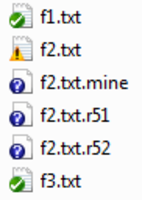
\includegraphics[width=0.3\textwidth, keepaspectratio]{iconFilesConflict.pdf}
  \caption{Files contents of the working directory during a conflict.}
  \label{fig:iconFileConflict}
\end{subfigure}
\caption{SVN icons for files in conflict state.}
\label{fig:systemIcons_4}
\end{figure}

\newpage


You will see that now the working folder has different files that you hadn't. In particular for this example they will become:


\begin{itemize}

	\item <file name>\footrednote{The "angle bracket" will exactly replace what is contained in. For example in case of the file name, it will be f2.txt.} with the yellow warning icon;
	
	\item <file name>.mine;
	
	\item <file name>.r<revision number of your local working folder>;
	
	\item <file name>.r<revision number on the remote repository>.

\end{itemize}


The third file in the directory (named \textit{f2.txt.mine}) contains what you just tried to commit.\\


The fourth one (named \textit{f2.txt.r51}) contains the revision you started to work on.\\

The second last file (named \textit{f2.txt.r52}) contains the last commit that you missed, and that is causing the conflict with your code line.\\

Finally the second file contains the same line of code taken from each previous file, and expressed as:

\begin{verbatim}

<<<<<<< .mine
const uint8_t string[] = "Right text";||||||| .r51
uint8_t string[] = "Text";=======
uint8_t string[] = "wrong text";>>>>>>> .r52
    
\end{verbatim}

The text contained between the symbols "<" and "=" is your updated text.\\
The text contained between "=" and ">" is the one updated by someone else and related to the revision specified at the end; in this case \textit{52}.\newline

To solve this conflict it is necessary to edit\footrednote{Yes! Manually!!!} the file removing \underline{all} the unwanted text; so in this case the previous block must be changed to:

\begin{verbatim}
    const uint8_t string[] = "Right text";
\end{verbatim}


To complete the conflict resolution it is necessary notify SVN that the conflict has been solved, using the \textit{resolve} option (figure \ref{fig:shellResolve}). A new window (figure \ref{fig:solveConflict}) will appear letting the user select which is the file to be marked as solved\footrednote{This is of course necessary in case of conflict on different files.}.\newline

\begin{figure}[htbp]
\begin{subfigure}{0.5\textwidth}
  \centering
  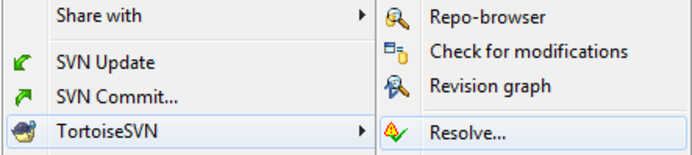
\includegraphics[width=\textwidth, keepaspectratio]{shellResolve.pdf}
  \caption{At the end of the conflict it is necessary communicate to SVN that the conflict has been solved.}
  \label{fig:shellResolve}
\end{subfigure}%
\begin{subfigure}{0.5\textwidth}
  \centering
  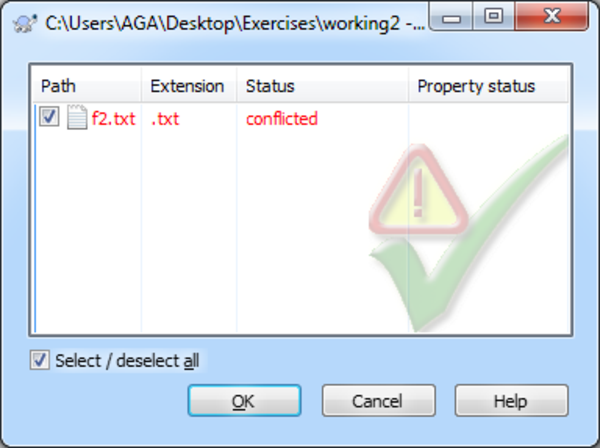
\includegraphics[width=0.7\textwidth, keepaspectratio]{solveConflict.pdf}
  \caption{A new window will let the user select the file to be declared solved .}
  \label{fig:solveConflict}
\end{subfigure}
\caption{To complete the procedure it is necessary confirm the accepted changes.}
\label{fig:solveConflicts}
\end{figure}

Another type of conflict that might arise, is when branches are merged.

Image that someone updated the main \textit{trunk} while you are working on the branch. If quite the same part of code is changed, as we saw, this might led to a conflict.\\


In this case, when we know that the right code lie in the local repository, or in another branch we can directly choose the relative button (\textit{Prefer local} or \textit{Prefer repository}) to accept the desired file version (figure \ref{fig:editConflict}).\\


\begin{figure}[ht!]
    \centering
    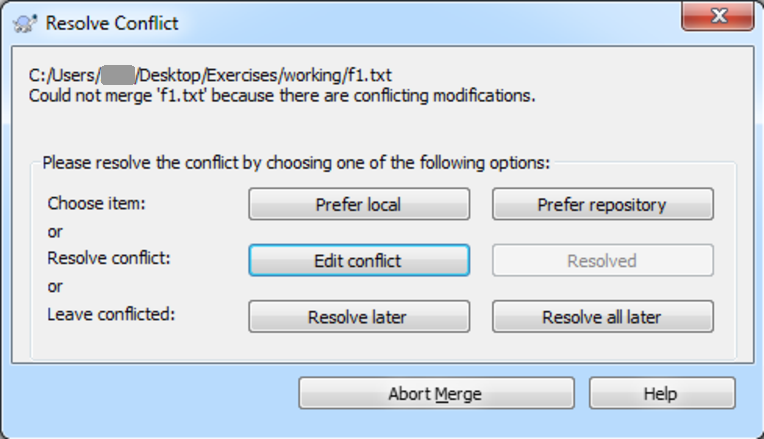
\includegraphics[width=0.6\textwidth, keepaspectratio]{editConflict.pdf}
    \caption{TortoiseSVN asks to the user to resolve the conflict.}
    \label{fig:editConflict}
\end{figure}


When we don't know what are the changes present in the other trunk we need to choose \textit{Edit conflict} and manually select the right lines of code as explained in the previous part.\\


In figure \ref{fig:tortoiseMerge}, similarly to the files in the previous example (figure \ref{fig:iconFileConflict}), are  showed the contents of the files in the repository (left side), the contents in the working folder (right side) and finally the merged result, that in this case needs to be updated by the user.\\

\begin{figure}[ht!]
    \centering
    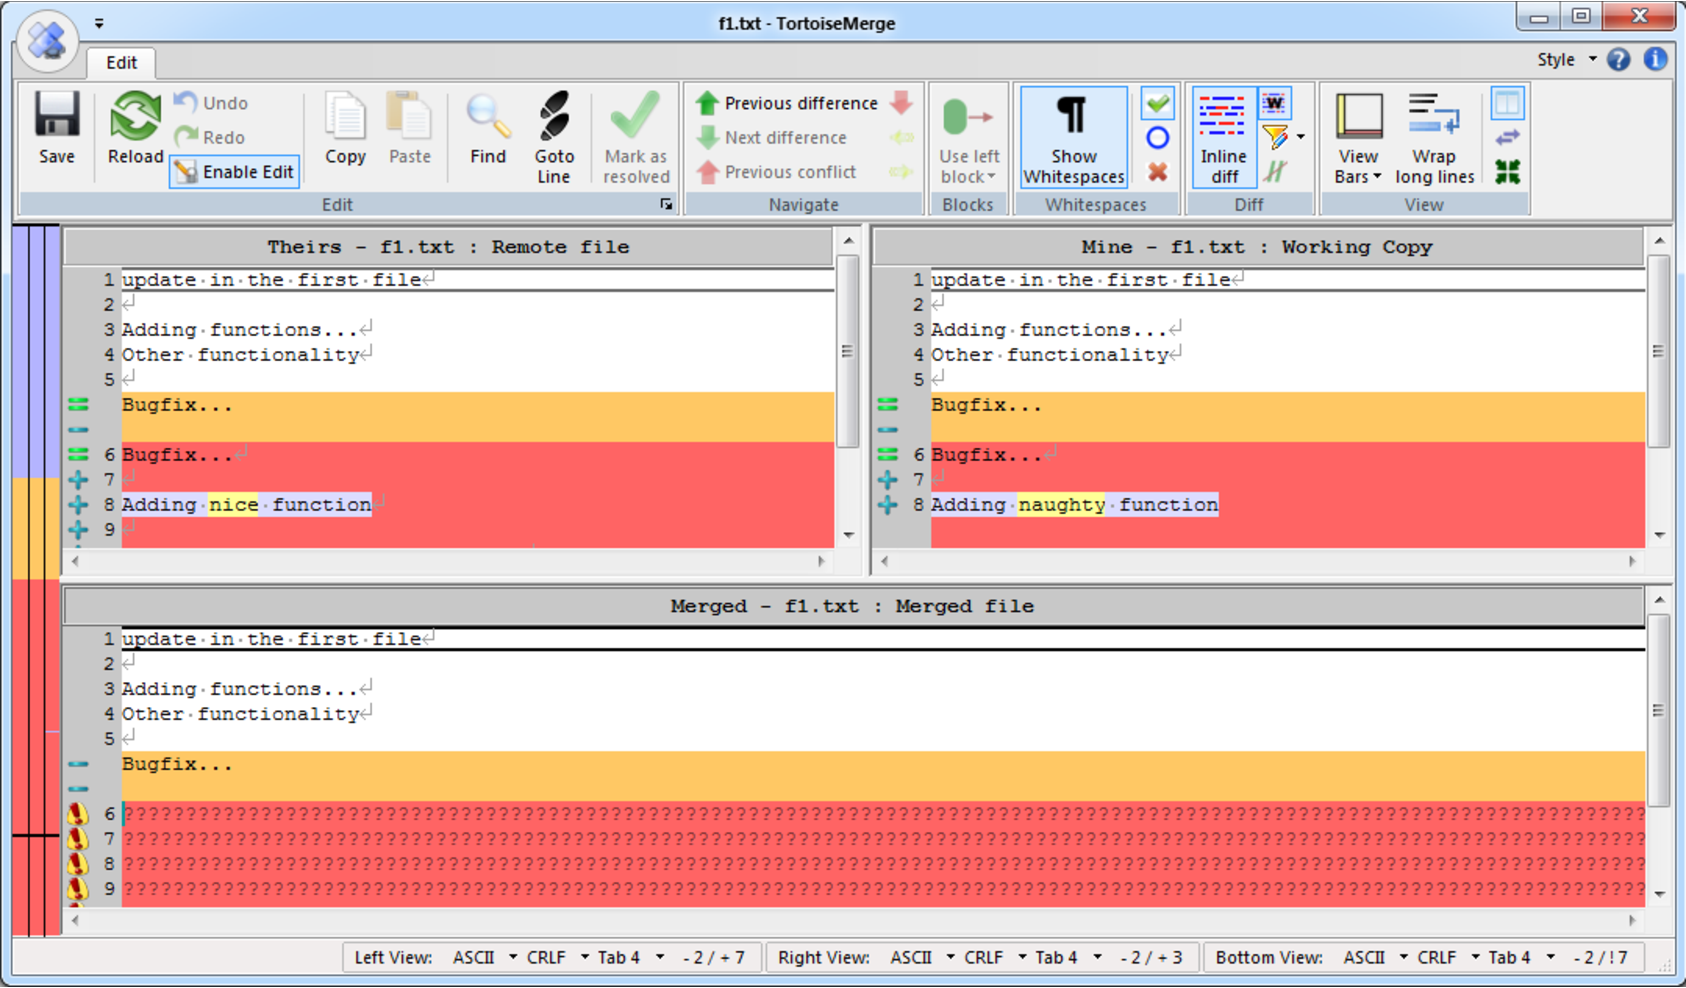
\includegraphics[width=\textwidth, keepaspectratio]{tortoiseMerge.pdf}
    \caption{TortoiseSVN show the conflict that prevent to merge the branch into the trunk.}
    \label{fig:tortoiseMerge}
\end{figure}

If for example we want to keep the text \textit{nice function} instead of the \textit{naughty function}, we can use the right click menu on the highlighted text and select the desired source. Even more it is possible keep the entry file from one source or from the other (figure \ref{fig:tortoiseResolve}).\\

\begin{figure}[ht!]
    \centering
    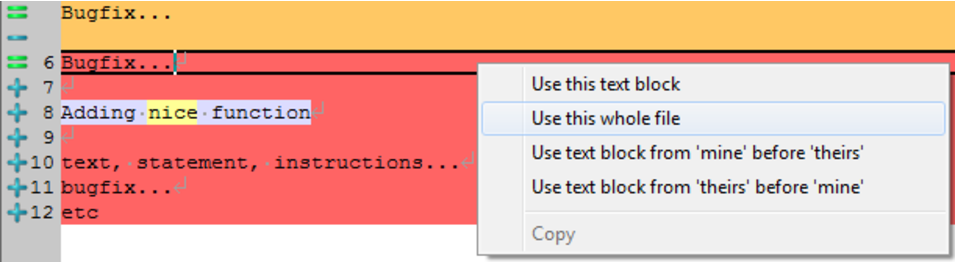
\includegraphics[width=\textwidth, keepaspectratio]{tortoiseResolve.pdf}
    \caption{TortoiseSVN allows to select the desired line of code from both file versions.}
    \label{fig:tortoiseResolve}
\end{figure}

Obviously it is also possible select mixed line of code from both file versions, the bottom window contains what in the end will be committed.

When the merge is completed, save the changes and close the editor.

Lastly, to complete the merge, select the the button \textit{Resolved} in the conflict window (\hbox{figure \ref{fig:editConflict}}) that now should be enabled.

\newpage










\subsection{Tag a software release}
\label{subsection:tagSoftwareRelease}

Every time you create a stable software that you want to release, you might take note of which commit is, or rather, tag that commit. This will create in the \textit{Tags} folder only well defined working software versions.\\

To tag a software version we have to proceed quite as we did to make a branch:

\begin{itemize}

    \item Update the working folder at the desired release version.

    \item Select the folder, then choose \textit{TortoiseSVN} $\rightarrow$ \textit{Branch/tag...} option from the menu (figure \ref{fig:shellCreateBranch}), a new pop-up window will appear (figure \ref{fig:tagVersion}).
    
    \item To create a tagged software, point the field \textit{To path:} \textit{/tags/<release name}\footrednote{For example 1.0.0.}> and in this case, select the radio button: \textit{Specific revision in repository}. This is necessary to "link" the desired revision with the passed tag name.
    
\end{itemize}




\begin{figure}[htbp]
\begin{subfigure}{0.5\textwidth}
  \centering
    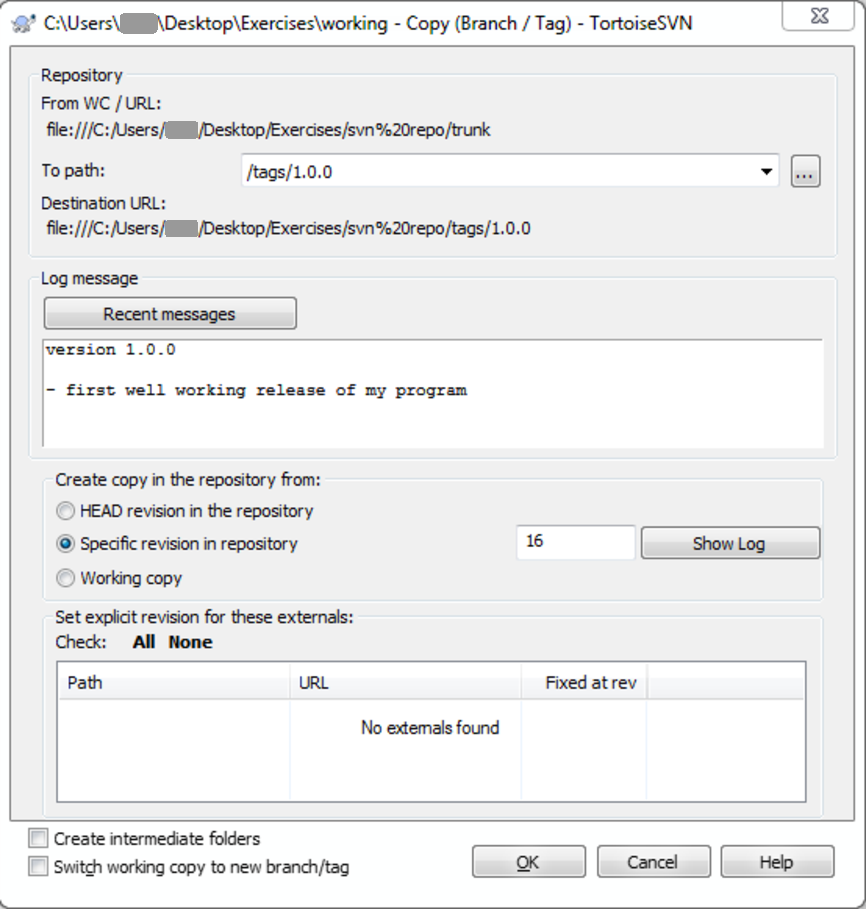
\includegraphics[width=\textwidth, keepaspectratio]{tagVersion.pdf}
    \caption{Tag a certain software version to be released.}
    \label{fig:tagVersion}
\end{subfigure}%
%\hspace{2mm}
\begin{subfigure}{0.5\textwidth}
  \centering
    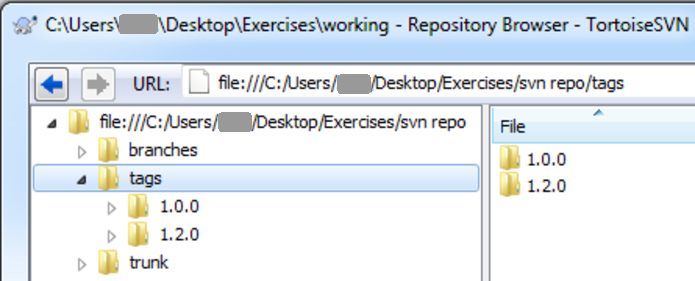
\includegraphics[width=0.85\textwidth, keepaspectratio]{tagSwVersions.pdf}
    \caption{Folders containing released software version.}
    \label{fig:tagSwVersions}
\end{subfigure}%
\caption{}
\label{fig:tagVersionWindows}
\end{figure}


\newpage
Now you end up with a similar situation reported in figure \ref{fig:tagSwVersions}, where every release has its own folder; in this way you will have always at hand the desired software version. You can also add an eventual release note file that contains all details of that version.






\section{Advanced functions}
\label{section:AdvancedFunctions}

In this section I will present just some useful functions to use in Subversion. These are not complicated concepts, but something over and above the typical normal use.






\subsection{Include externals}
\label{subsection:externals}

In some cases it might be really useful pack more repository together, to reuse something that you developed in the past, or to organize a work that has heterogeneous repositories.\\

For example, let's say that we want to add a new functionality to our project using a library (that has its own repository) previously developed.

To quickly solve the problem we could just copy these files into the project folder, or to solve it brilliantly, we might use the \textit{externals} project properties.


This function links the library and the project repositories together, to end up with a commit that includes every necessary files to build the project (figure \ref{fig:svnExternalsFlow}).\\






\begin{figure}[htbp]
    \centering
    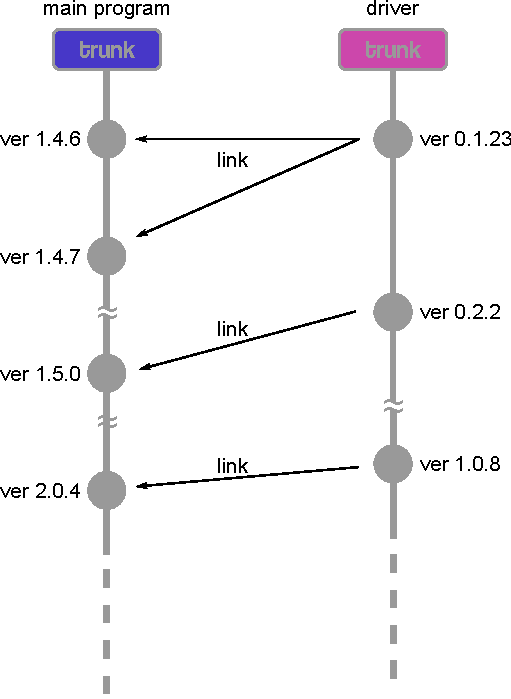
\includegraphics[width=0.45\textwidth, keepaspectratio]{svnExternalsFlow.pdf}
    \caption{SVN with its \textit{externals} property allows to link different commits from various repositories.}
    \label{fig:svnExternalsFlow}
\end{figure}







To test this functionality we need to create another repository (named \textit{svn repo lib}) and its working folder (named \textit{library}) (figure \ref{fig:iconExternalsProject}).





\newpage

Here the steps to apply the \textit{externals} project properties on our example:



\begin{itemize}

    \item Open the SVN properties on the project folder (\textit{working}): \textit{TortoiseSVN} $\rightarrow$ \textit{Properties} (figure \ref{fig:shellProperties}).
    
    \item In the new window select: \textit{New} $\rightarrow$ \textit{Externals} (figure \ref{fig:newExternals}), a pop-up window will appear to let you insert the external repository (figure \ref{fig:addExternals}).
    
    \item In this new window press the button \textit{New} again and a pop-up will allow you to insert the path to the external repository and its details for the desired commit (figure \ref{fig:addExternals}).\newline
    
    In that window you will see the following fields:
    
    \begin{description}
    
        \item[Local path]: is \underline{the name} of the directory that will be created inside the project folder to contain the external committed files. For the example, this is named: \textit{Driver} (figure \ref{fig:addExternals}).
        
        \item[URL]: is the path to the external repository. Use \textit{Repo-browser} to correctly find the desired folder. In this case I'm pointing to the \textit{trunk} of the external library repository.
        
        \item[Revision]: can be any commit. Use the radio button to choose the last (\textit{HEAD revision}) or any other (\textit{Revision}). In this case I pointed to a certain library version.
    
    \end{description}
    
    \item Finally to conclude the operation it is necessary to execute the update (to checkout the \textit{externals} files in the project directory), and the commit command to finalise the application of the external properties to the project folder (figure \ref{fig:iconExternalsFiles}).
    
    
\end{itemize}








\begin{figure}[htbp]
\begin{subfigure}{0.45\textwidth}
  \centering
  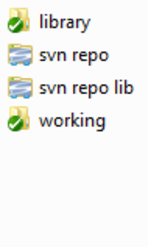
\includegraphics[width=0.35\textwidth, keepaspectratio]{iconExternalsProject.pdf}
  \caption{Folders of a project linked to an externals properties.}
  \label{fig:iconExternalsProject}
\end{subfigure}%
\hspace{5mm}
\begin{subfigure}{0.45\textwidth}
  \centering
  
\includegraphics[width=0.25\textwidth, keepaspectratio]{iconExternalsFiles.pdf}
  \caption{Commit files of a project using an externals repository.}
  \label{fig:iconExternalsFiles}
\end{subfigure}
\caption{Folders and files related to the example.}
\label{fig:svnExternalsIcons}
\end{figure}
 


\begin{figure}[htbp]
    \centering
    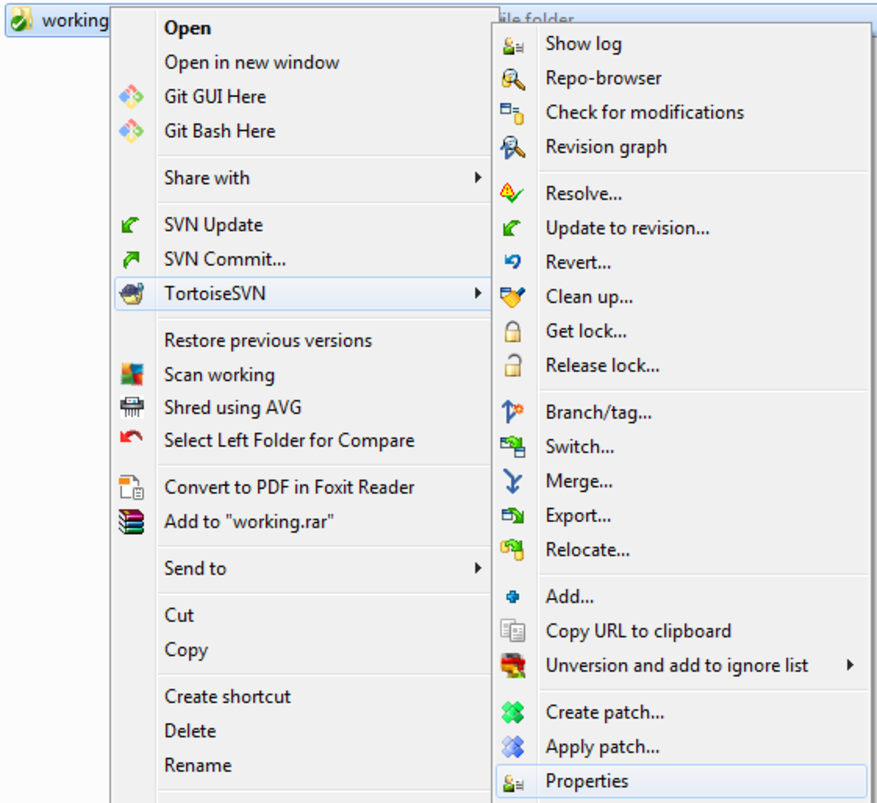
\includegraphics[width=0.65\textwidth, keepaspectratio]{shellProperties.pdf}
    \caption{Open project properties.}
    \label{fig:shellProperties}
\end{figure}


\begin{figure}[htbp]
    \centering
    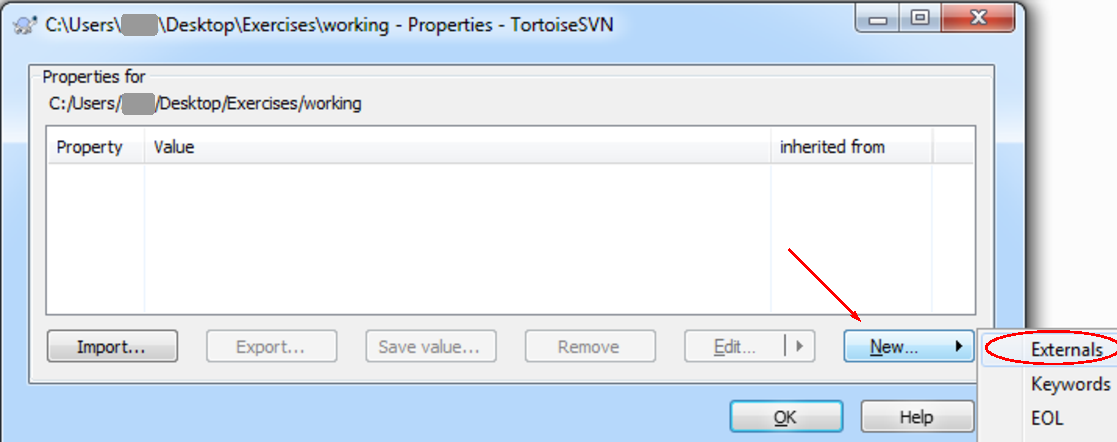
\includegraphics[width=0.65\textwidth, keepaspectratio]{newExternals.pdf}
    \caption{Select the repository properties.}
    \label{fig:newExternals}
\end{figure}


\begin{figure}[htbp]
    \centering
    \includegraphics[width=0.65\textwidth, keepaspectratio]{addExternals.pdf}
    \caption{Add a new external and specify all the details related to the "linked" repository.}
    \label{fig:addExternals}
\end{figure}

\fbox{\begin{minipage}{\textwidth}

\textbf{Pay attention:}\vspace{1mm}

If you select the \textit{HEAD revision} option (figure \ref{fig:addExternals}) the \textit{externals} included will always point to the last commit of that repository.\vspace{2mm}

To use a fixed version select the \textit{Revision} option and pick-up the desired commit through the \textit{Show log} button. \underline{This is by far the suggested option to use}.\\

Using the \textit{HEAD revision} option you have to take in account even another point:

\begin{itemize}

    \item If the \textit{externals} (\textit{Driver} folder) has a repository (\textit{svn repo lib}) located in the same project repository (\textit{svn repo} folder), any commit done to the library (\textit{library} folder) will be reflected also in the linked folder present in the project (\textit{driver} folder) at the commit time.
    
    \item If the \textit{externals} (\textit{Driver} folder) has a repository (\textit{svn repo lib}) located on a different path (as we did in this example), any commit done to the library will be notified at the time to commit the project (\textit{working} folder), then to keep the externals up-to-date the user must update first the project folder before committing the entry project\footrednote{This is what I found in the \href{https://tortoisesvn.net/docs/release/TortoiseSVN_en/tsvn-dug-externals.html}{official documentation}, however when I tested it, its behaviour has been as it had would been in the same project repository. Actually this is a bug, I checked the \href{https://tortoisesvn.net/Changelog.txt}{changelog file}.}.

\end{itemize}

\end{minipage}}

\vspace{5mm}

The \textit{externals} can be identified even from the repo-browser. They appear with an icon (a blue arrow) which remember the \textit{Windows OS} shortcut system icon (figure \ref{fig:externalsRepoBrowser}).


\begin{figure}[htbp]
    \centering
    \includegraphics[width=0.65\textwidth, keepaspectratio]{externalsRepoBrowser.pdf}
    \caption{The externals files/folders are showed in the repo-browser with a different icon.}
    \label{fig:externalsRepoBrowser}
\end{figure}









\subsection{Lock a file}
\label{subsection:lockFile}

In some cases, before starting to work on a file, it is convenient to keep lock on it while editing.

When the project is shared between people, there is a chance that more than one person is trying to edit the same file, as seen, this might give rise to conflicts.\\

If this is text file there should be fewer issues with multiple editors (as seen in section \ref{subsection:ResolveConflicts}), but if this is a binary file (such a CAD format), then merging multiple updates is likely to corrupt the file.\\


To avoid this situation only one person at time should update that types of file.

In this case it is suggested to use the SVN lock file function.\\ 

Before starting to work on a file you should lock it so that other users cannot commit their changes until you have committed yours or voluntarily relinquished the lock.\\

To lock a file:

\begin{itemize}

    \item Select the file to be locked then choose: \textit{TortoiseSVN} $\rightarrow$ \textit{Get lock...} (figure \ref{fig:shellLock}).
    
    \item A new window will appear asking the user to insert an optional message that will be showed to users that try to commit changes on the same file (figure \ref{fig:lockMessage}).
    
    \item At the end of your work, as soon as you'll commit the job, the lock will be automatically released. If, for some reason you want keep the file still locked you have to check the box \textit{Keep locks} visible in figure \ref{fig:keepLock}.
    
\end{itemize}





\begin{figure}[htbp]
    \centering
    \includegraphics[width=0.5\textwidth, keepaspectratio]{shellLock.pdf}
    \caption{Before start to work use the TortoiseSVN menu to lock the file.}
    \label{fig:shellLock}
\end{figure}



\begin{figure}[htbp]
\begin{subfigure}{0.5\textwidth}
  \centering
  \includegraphics[width=0.98\textwidth, keepaspectratio]{lockMessage.pdf}
  \caption{Let other users know who is locking the file inserting a meaningful message.}
  \label{fig:lockMessage}
\end{subfigure}%
\hspace{5mm}
\begin{subfigure}{0.5\textwidth}
  \centering
  \includegraphics[width=0.94\textwidth, keepaspectratio]{keepLock.pdf}
  \caption{At the commit time the user can decide if release the file or continue to keep it lock it.}
  \label{fig:keepLock}
\end{subfigure}
\caption{SVN locking function.}
\label{fig:svnLocks}
\end{figure}



This mechanism for sure can prevent to corrupt files, but it can't save the users from wasting their time.\newline

In fact suppose that for a misunderstanding, you and a your colleague start to work at the same time on the same binary file; he locks the file, but you forget to do it. After hours of hard work, you are proud to commit your job, but soon you realise what's happened. $\skull \skull \skull$\\

Is it possible to prevent this scenario? Yes it is.\\

Subversion has a property that force all working files to be read only (in their default state), except when a lock is applied to a file. In this situation the user will be forced to lock the file before to start to work on it, thus making the file editing mutually exclusive.\newline

To apply this property it is necessary to proceed as we did to apply the \textit{externals}, but of course selecting this other.

\begin{itemize}

    \item Select the working folder and then \textit{TortoiseSVN} $\rightarrow$ \textit{Properties} (figure \ref{fig:shellProperties}).
    
    \item In the new window choose \textit{New}, and select \textit{Needs-Lock} from the drop-down menu (\ref{fig:needsLockProperties}).
    
    \item A new dialog box (figure \ref{fig:readOnlyLock}) will let the user select which kind of lock is required. To make the project file read only as default, choose the option \textit{Locking required(read-only update)} and confirm.
    
\end{itemize}




\begin{figure}[htbp]
\begin{subfigure}{0.5\textwidth}
  \centering
  \includegraphics[width=0.98\textwidth, keepaspectratio]{needsLockProperties.pdf}
  \caption{Add the Needs-Lock property to the project.}
  \label{fig:needsLockProperties}
\end{subfigure}%
\hspace{5mm}
\begin{subfigure}{0.5\textwidth}
  \centering
  \includegraphics[width=0.94\textwidth, keepaspectratio]{readOnlyLock.pdf}
  \caption{To make the file editing mutually exclusive select the first option.}
  \label{fig:readOnlyLock}
\end{subfigure}
\caption{SVN locking function.}
\label{fig:svnKeepLocks}
\end{figure}

Now all files in the working directory are read only. This should be displayed by the gray icon instead of the green one. Unfortunately due to a \href{http://tortoisesvn.tigris.org/faq.html#ovlnotall}{limitation} of the \textit{Microsoft OS} this, doesn't work\footrednote{To see all the available icons go to the \textit{TortoiseSVN} $\rightarrow$ \textit{Settings} and select the Icon Set submenu.}. To fix the problem a workaround exist, but it is more fast (and safe) just open the file and check if this is read/write.\\

Quite a number of text editor have an icon relating to the read/write state of the file, for example \textit{Notepad++} has an icon on the file tab whose the color depends on the file state: gray for read only and blue for a read/write file.\newline


To run this example is necessary to use another "user" from the same machine or a different machine, and of course, create a repository accessible from both users. Create then a local working folder that point to this common repository.\\

\begin{itemize}

    \item Lock the file you want to start to work on.
    
    \item Change user and try to lock the same file. In this case, before starting to consume your time you'll been advised that the file has already been locked by the other user (figure \ref{fig:errorFileLocked}).

\end{itemize}




\begin{figure}[htbp]
    \centering
    \includegraphics[width=0.8\textwidth, keepaspectratio]{errorFileLocked.pdf}
    \caption{When another user locked the file you can't even start to working on it, this will save you some time.}
    \label{fig:errorFileLocked}
\end{figure}





To find out more refer to the \href{https://tortoisesvn.net/docs/release/TortoiseSVN_en/tsvn-dug-locking.html}{official documentation}.








\subsection{Using SVN from command line}
\label{subsection:SVNCommandLine}

When you need to automate a process, TortoiseSVN shell is not more suitable, 
in this case you need to use the SVN command line.\newline


To verify your SVN command line installation: Open the \textit{command window} in the working directory and launch the command: \textit{svn info}.

%%%%%%%%%%%%%%%%%%%%%%%%%%%%%%%%%%%%%%%%%%%%%%%%%%%%%%%%%%%%%%%%%%%%%%%%%%%
%%%%%%%%%%%%%%%%%%%%%% CHECK THE SVN INFO %%%%%%%%%%%%%%%%%%%%
\lstinputlisting[style=DOS,
caption={Output of the \textit{svn info} command in the working directory}, %
label=lst:svnTest, %
firstline=1, lastline=13]{srcCode/svnCommands.txt}
%%%%%%%%%%%%%%%%%%%%%%%%%%%%%%%%%%%%%%%%%%%%%%%%%%%%%%%%%%%%%%%%%%%%%%%%%%%

If you get a similar output of the list \ref{lst:svnTest}, then you are ready, but if you get an error, you miss the installation of that feature. To install it refer to section \ref{subsection:InstallSoftware}.

If you still have the same problem you might have to add the SVN command to the path\footrednote{See section \ref{subsection:systemPath}.} environment variables.

\subsubsection{Commands}

Below (list \ref{lst:svnAllCommands}) I reported some of the most used SVN commands to successfully manage a project creating your custom functions.

\begin{itemize}

\item \textbf{add} files or directories to the working folder;

\item \textbf{commit} the working folder;

\item \textbf{revert} the selected file, or the whole working folder;

\item \textbf{update} the selected file, or the whole working folder;

\item \textbf{checkout} the repository at the last or at the passed revision;

\item \textbf{extract} the desired file from repository in the present folder

\end{itemize}

To get the complete list of the available SVN functions see the \href{http://svnbook.red-bean.com/en/1.7/svn.ref.html}{official documentation}.

%%%%%%%%%%%%%%%%%%%%%%%%%%%%%%%%%%%%%%%%%%%%%%%%%%%%%%%%%%%%%%%%%%%%%%%%%%%
%%%%%%%%%%%%%%%%%%%%%% SVN ALL CMD %%%%%%%%%%%%%%%%%%%%
\lstinputlisting[style=DOS,
caption={SVN commands to manage the files projects}, %
label=lst:svnAllCommands, %
firstline=17, lastline=39]{srcCode/svnCommands.txt}
%%%%%%%%%%%%%%%%%%%%%%%%%%%%%%%%%%%%%%%%%%%%%%%%%%%%%%%%%%%%%%%%%%%%%%%%%%%

In some cases, like before a commit, you might want to make appear a dialog box.

You can do easily invoking the TortoiseSVN shell\footrednote{To find out more visit the \href{https://tortoisesvn.net/docs/nightly/TortoiseSVN_en/tsvn-automation.html}{official page}.}.\newline

In list \ref{lst:TortoiseSVNCommitCommand} is reported the command to launch the TortoiseSVN commit command for the working folder used in the previous examples.


%%%%%%%%%%%%%%%%%%%%%%%%%%%%%%%%%%%%%%%%%%%%%%%%%%%%%%%%%%%%%%%%%%%%%%%%%%%
%%%%%%%%%%%%%%%%%%%%%% TortoiseSVN commit %%%%%%%%%%%%%%%%%%%%
\lstinputlisting[style=DOS,
caption={TortoiseSVN command to invoke the commit window.}, %
label=lst:TortoiseSVNCommitCommand, %
firstline=43, lastline=44]{srcCode/svnCommands.txt}
%%%%%%%%%%%%%%%%%%%%%%%%%%%%%%%%%%%%%%%%%%%%%%%%%%%%%%%%%%%%%%%%%%%%%%%%%%%

You will see appear the same window that you see when you call the commit from the shell (figure \ref{fig:commitMessage}).



Of course it has not really sense to launch these command from the system \textit{cmd} when you have the shell. These are in fact useful when you have a program that need to interact with SVN (like a Python script).

To show you how to use these commands I created a Python function to invoke the commit command in both versions: using TortoiseSVN and using the SVN command line (list \ref{lst:PythonCommitFunction}).


\newpage

%%%%%%%%%%%%%%%%%%%%%%%%%%%%%%%%%%%%%%%%%%%%%%%%%%%%%%%%%%%%%%%%%%%%%%%%%%%
%%%%%%%%%%%%%%%%%%%%%% Python commit function %%%%%%%%%%%%%%%%%%%
\lstinputlisting[style=Python,
caption={User function made in Python to launch the commit command.}, %
label=lst:PythonCommitFunction, %
firstline=48, lastline=79]{srcCode/svnCommands.txt}
%%%%%%%%%%%%%%%%%%%%%%%%%%%%%%%%%%%%%%%%%%%%%%%%%%%%%%%%%%%%%%%%%%%%%%%%%%%



\newpage












\section{Fast help and suggestions}
\label{fastHelp}


\subsection{Common mistakes}
\label{section:commonMistakes}

Either you're new or not to a version control system you may incur in some common mistakes, here a quick troubleshooting list:

\begin{itemize}

    \item working files don't update;
    \item I can't delete project files;
    \item I can't rename a file correctly;
    \item write a commit log.
    
\end{itemize}







\subsubsection{Working files don't update}
\label{subsubsection:UpdateNotWork}

\textit{I'm trying to update the local folder to the last or selected commit, but files still remain at the same point.}\newline

Every time you modify a versioned file, imagine what happens if instead of committing all your hard work, you press the updated button by mistake and the system resets all changes? $\skull \skull \skull$.\\


This is the reason why, when you press the \textit{update} button the selected files or the entire folder doesn't discard the last updates. In this case to discard the last modification you should execute the shell \textit{Revert} command (section \ref{subsection:revertFiles}).\\


If you are still in trouble and there is a "mess" in the folder you can also delete all\footrednote{Pay attention, you are going to loose all your changes.} the contents and then run \textit{SVN Update} (figure \ref{fig:iconWorkingUpdated}). This will remove all the files (edited and not) that might create a conflict. The update command will "download" in your working directory all the files related to the last commit.














\subsubsection{I Can't delete project files}
\label{subsubsection:DeleteProjectFiles}

\textit{I tried to delete some working files, but after an update they are still present.}\newline


If you have a project that might evolve in a different way (sometime files are added, sometime files are removed) you have to delete these project files in the same way as you added them, that is using the TortoiseSVN shell.

\begin{itemize}
    
    \item Select the file that you want to remove and choose: \textit{TortoiseSVN} $\rightarrow$ \textit{Delete} (figure \ref{fig:shellDelete}).
    
\end{itemize}



\begin{figure}[ht!]
    \centering
    \includegraphics[width=0.5\textwidth, keepaspectratio]{shellDelete.pdf}
    \caption{To delete the project files you have to use the TortoiseSVN shell.}
    \label{fig:shellDelete}
\end{figure}


Now that file will be no longer "linked" to the VCS. If you only would delete the files from the working directory without using the SVN command, these files would still be part of the project. That explain why every time you use the update command, the version control system download also them.





\subsubsection{I can't rename a file correctly}
\label{subsubsection:RenameFile}

\textit{I tried to rename a file, but it doesn't look under version control, and when I update the old file still exist\ldots}\newline

This is correct, since you renamed the file using the system command and not SVN. I'll try to show you why.
For example, you want to rename the file \textit{f2.txt} that is actually under version control, since has been added at the project creation. Now, using the Windows shell, you rename it to \textit{fileFunction.c}. At this point SVN doesn't see anymore that file, it is like it was deleted, so in case of the \textit{update} command, this will be copied again to the working folder. Even more the renamed file is not under version control. As you might have guessed to rename the file you have to use the TortoiseSVN shell. This operation can be thought as a series of these commands: \textbf{remove} the file \textit{f2.txt} from the version control system, rename the file to \textit{fileFunction.c} and finally \textbf{adding} it to Subversion.










\subsubsection{Write a commit log}
\label{subsubsectio:HowWriteRevision}


\textit{How should I write a commit log?}\newline

Probably this is a question that, like me, many of you had had. I tried a lot of different methods and I searched online for useful advice, and in time I think that I arrived up to 90\% of the job. A friend of mine (Matt) gave me the remain 10\%! $\smileface$.

I'll try to explain what work for me, but of course, there isn't a right rule, so you can personalise it how do prefer.

The only important thing is that the message \underline{will be clear and self explanatory} about what you made in that commit.\\

So what I use? I divide the message in two parts: 

\begin{enumerate}

    \item the version number;
    
    \item the changes done in that commit.
    
\end{enumerate}


The version number follow \href{https://semver.org/}{this} schema\footrednote{Thanks to Matthew C.!!!}: \textbf{MajorNumber}.\textbf{MinorNumber}.\textbf{PatchNumber} where:

\begin{description}

    \item [Major number] this number must be incremented when an incompatible change is done;
    
    \item [Minor number] this number must be incremented when you a functionality that is backwards compatible;
    
    \item [Patch number] this number must be incremented when a bugfix or a compatible function is added.
    
\end{description}


After this version number I insert a general overview of what I did, then in the follow lines I describe point per point what changed and what I added or removed. The text is always lower case (except few exception) using these keywords:


\begin{description}

    \item [added] when a file/function has been added;
    
    \item [updated] when a file function has been changed;
    
    \item [removed] when a file/function has been removed;
    
    \item [fixed] when a bug is resolved.

\end{description}


Here some examples:

\begin{verbatim}
    0.0.1 - project started
    - created the repository
    - added the files "f1.txt", "f2.txt" at the working folder
\end{verbatim}

\begin{verbatim}
    0.1.22 - started to create the function "readTemperature" - work in progress
    - added the I2C driver to read temperature from sensors
    - updated the function "readTemperature", now convert to degC
\end{verbatim}

\begin{verbatim}
    0.2.0 - completed the chapter 3
    - fixed the chapter typos
    - updated the list of components
    - removed the section about the pipe
\end{verbatim}

\ \\













\subsection{Useful suggestions}
\label{section:UsefulSuggestions}

Here I grouped some tips that might be useful to use and to understand Subversion better.


\begin{itemize}
    
    \item I want to see the project history and its commit messages;
    \item I want to change the commit message;
    \item I noted that every file has its own version, why?;
    \item I would like to share a SVN project with friends;
    \item add a program to system PATH environment variables;
    \item is there a "cheatsheet" related to the VCS workflow?
    
\end{itemize}


\subsubsection{I want to see the project history and its commit messages}
\label{subsubsectio:ProjectHisory}

To view all the project history you can use the \textit{Show log} option from the \textit{TortoiseSVN} menu on the working dir. Through this menu (figure \ref{fig:selectCommitRevision}) you can see all the commits, the revision number, its message and the files committed.


\subsubsection{I want to change the commit message}
\label{subsubsection:EditCommitMessage}


\textit{I made a mistake writing a commit message.} \newline


SVN has the ability to let the user update the commit message. This function can be useful in case of typo or to add forgot details to a commit.\newline

\begin{itemize}

    \item Select the commit you want to edit from the \textit{Log Messages} window and with the right click choose the option \textit{Edit log message} from the drop-down menu (figure \ref{fig:logMessages}).
    
    \item A pop-up window will appear, that lets you change the commit message. Edit the message and confirm.
    
\end{itemize}

Very likely you'll receive an error message (figure \ref{fig:errorEditMsg}), this is due to a protection in the SVN configuration files, classic of a default system configuration.





\begin{figure}[htbp]
\begin{subfigure}{0.5\textwidth}
  \centering
  \includegraphics[width=0.7\textwidth, keepaspectratio]{logMessages.pdf}
  \caption{From the drop-down menu select the \hbox{\textit{Edit log message}} option.}
  \label{fig:logMessages}
\end{subfigure}%
\hspace{5mm}
\begin{subfigure}{0.5\textwidth}
  \centering
  \includegraphics[width=0.7\textwidth, keepaspectratio]{errorEditMsg.pdf}
  \caption{On a default installation you can't edit the commit message.}
  \label{fig:errorEditMsg}
\end{subfigure}
\caption{}
\label{fig:svnEditLogMsg}
\end{figure}


\newpage

To enable this feature:

\begin{itemize}

    \item Find the file \textit{pre-revprop-change.tmpl} located at the path: \textit{<yourSVNRepositoryFolder>/hooks}\footrednote{In my case is: \textit{C:/Users/AleTheCoder/Desktop/Exercises/svn repo/hooks}.}
    
    \item Rename the file extension from \textit{*.tmpl} to \textit{*.bat}.
    
    \item As in the example below, (list \ref{lst:enableEditLogMsg}) comment the code related to the changing properties, and add the last two line.
    
\end{itemize}


%%%%%%%%%%%%%%%%%%%%%%%%%%%%%%%%%%%%%%%%%%%%%%%%%%%%%%%%%%%%%%%%%%%%%%%%%%%
%%%%%%%%%%%%%%%%%%%%%% EDIT THE SVN PROPERTY %%%%%%%%%%%%%%%%%%%%
\lstinputlisting[style=DOS,
caption={Content of the file \textit{pre-revprop-change.bat after the "update".}}, %
label=lst:enableEditLogMsg, %
firstline=82, lastline=90]{srcCode/svnCommands.txt}
%%%%%%%%%%%%%%%%%%%%%%%%%%%%%%%%%%%%%%%%%%%%%%%%%%%%%%%%%%%%%%%%%%%%%%%%%%%

If the file has been changed properly, re-executing the previous steps will now change the commit message.







\subsubsection{I noted that every file has its own version, why?}
\label{subsubsectio:FileVersion}

In figure \ref{fig:svnCommitWorkflow} is reported how a version control works without deeply discuss the way that SVN uses to version the project files.
The following diagram (figure \ref{fig:svnFilesVersion}) explain how Subversion "tags" a file with a certain number. We see that this match the commit number (of the project) where it took part. That explains why some file look up-to-date, and others not. You can easily check these numbers comparing the \textit{Log Messages} window and the \textit{Repository Browser} (figure \ref{fig:logMsgVsRepoBrowser})



\begin{figure}[htbp]
    \centering
    \includegraphics[width=\textwidth, keepaspectratio]{svnFilesVersion.pdf}
    \caption{This is the way how Subversion tags files version.}
    \label{fig:svnFilesVersion}
\end{figure}


%\vspace{25.00mm}


\begin{figure}[htbp]
    \centering
    \includegraphics[width=\textwidth, keepaspectratio]{logMsgVsRepoBrowser.pdf}
    \caption{Here is showed how Subversion tags files version.}
    \label{fig:logMsgVsRepoBrowser}
\end{figure}

\newpage

\subsubsection{I would like to share a SVN project with friends}
\label{subsubsectio:SvnAtHome}

\textit{I would like to use Subversion at home for my stuff, but of course I don't have a server. How can I do?}\newline

When you want to use SVN at home you could create the a local repository as seen for the example, but of course this is not safe, so this is not the best option.

In this case you might want to use a cloud service like: \href{https://riouxsvn.com/}{RiouxSVN} (figure \ref{fig:riouxWebsite}) with this you can create and use your own repository. Of course it also possible let other members collaborate to your project.



\begin{figure}[ht!]
    \centering
    \includegraphics[width=\textwidth, keepaspectratio]{riouxWebsite.pdf}
    \caption{Some cloud services allow you to use SVN for your personal projects.}
    \label{fig:riouxWebsite}
\end{figure}

If you want, you can even use a domestic NAS\footrednote{Network Archive Storage.} or create a new one using a microcomputer like Banana Pi\ldots The NET it's plenty of tutorial on these kind of arguments.



\newpage

\subsection{Add a program to system PATH environment variables}
\label{subsection:systemPath}

When you install a fresh copy of the operating system your command window \textit{knows} only commands belonging to the standard Windows OS.

If a new program is installed and you want make it run from the command window, you have to \textit{register} it into the system.\newline

Open the Windows \textit{Control panel} and choose \textit{System}, then select \textit{Advanced system setting} and a new window will appear (figure \ref{fig:openEnvironmentVariables}).


\begin{figure}[htbp]
\begin{subfigure}{0.5\textwidth}
  \centering
  \includegraphics[width=0.97\textwidth, keepaspectratio]{openEnvironmentVariables.pdf}
  \caption{Open the environment variables.}
  \label{fig:openEnvironmentVariables}
\end{subfigure}%
\hspace{5mm}
\begin{subfigure}{0.5\textwidth}
  \centering
  \includegraphics[width=0.7\textwidth, keepaspectratio]{editSystemPath.pdf}
  \caption{Add TortoiseSVN to the system path.}
  \label{fig:editSystemPath}
\end{subfigure}
\caption{}
\label{fig:addPath}
\end{figure}





In the tab \textit{Advanced} choose the \textit{Environment Variables...} button, a new window will appear again (figure \ref{fig:editSystemPath}).

Under the panel \textit{System variables} find the variable \textit{Path} and edit the string, appending at the end of the existing line, the path to the executable program to add. 

\underline{Remember the semicolon} before add your path! The line should looks like list \ref{lst:SystemPath}.

%%%%%%%%%%%%%%%%%%%%%%%%%%%%%%%%%%%%%%%%%%%%%%%%%%%%%%%%%%%%%%%%%%%%%%%%%%%
%%%%%%%%%%%%%%%%%%%%%% Windows system path %%%%%%%%%%%%%%%%%%%
\lstinputlisting[style=DOS,
caption={Example of the path variable.}, %
label=lst:SystemPath, %
firstline=93, lastline=93]{srcCode/svnCommands.txt}
%%%%%%%%%%%%%%%%%%%%%%%%%%%%%%%%%%%%%%%%%%%%%%%%%%%%%%%%%%%%%%%%%%%%%%%%%%%

Confirm the changes and restart the command window (\textit{cmd}), you should now be able to launch the program added.




\subsection{Is there a "cheatsheet" related to the VCS workflow?}
\label{subsection:cheatsheet}

Yes there is! On the next page you will find an useful (I hope) graph showing how use a version control system on your projects.\newline

Ale theCoder


Ver 1.0\ \\


Thanks to \LaTeXe


\newpage


\begin{landscape}
\thispagestyle{empty}
    \centering
    \includegraphics[keepaspectratio]{svnSummaryFlow.pdf}
    %\caption{Some cloud service allow you to use SVN for your personal project.}
    %\label{fig:riouxWebsite}
%\end{sidewaysfigure}
\end{landscape}








